%#################################################################
\chapter{Avaliação Experimental}\label{validacaoProposta}
%#################################################################
Este capítulo apresenta o experimento controlado que foi executado com a finalidade de verificar a viabilidade de uso da solução desenvolvida neste trabalho. 
Foram realizadas atividades que envolveram a execução de práticas de modelagem comparando os resultados da proposta deste estudo com a abordagem gráfica do BrModelo, uma ferramenta reconhecidamente utilizada no ensino de \acp{BD} nos cursos de graduação.

Sendo assim, foram realizadas análises quantitativas e qualitativas dos resultados coletados do experimento. 
Isso foi realizado a partir de métricas referentes ao esforço (tempo), precisão, revocação, Medida-F, bem como em questionários qualitativos para avaliação de itens referentes à utilidade percebida e facilidade de uso de ambas as abordagens.

A Seção \ref{sec:defExp} apresenta a definição da avaliação, seguida de seu escopo na Seção \ref{sec:escopoExp} e do planejamento na Seção \ref{ssec:planejExp}.
As atividades conduzidas na operação do experimento são relatadas na Seção \ref{ssec:operacaoExp}.
Finalmente, os resultados obtidos são apresentados na Seção \ref{sec:resultExp} e os lições do capítulo pontudas na Seção \ref{sec:licoesExp}.

%#################################################################
\section{Definição da Avaliação} \label{sec:defExp}
%#################################################################
Segundo \citeonline{Wohlin:2012}, a \ac{ESE} trata da utilização de abordagens científicas para o desenvolvimento, evolução, manutenção e validação de software. 
A \ac{ESE} usa métodos científicos para fazer pesquisa e para também tomar decisões sobre mudanças na forma de desenvolver software.

Na \ac{ESE} é possível realizar medições controladas, objetivas e orientadas a verificação, caracterizando assim a análise quantitativa. 
Da mesma forma, também é possível fazer observações naturalísticas, entrevistas e questionários, sendo essa uma abordagem orientada a descoberta e caracterizada como análise qualitativa.

As diferentes técnicas que a \ac{ESE} engloba podem ser classificadas em dois grandes grupos: estudos experimentais e observacionais. 
Enquanto nas técnicas observacionais o pesquisador conduz a investigação sobre um objeto de estudo sem qualquer ação sobre ele, nas técnicas experimentais existe essa intervenção pela inclusão, exclusão ou modificação de algum fator estudado, procurando comparar o comportamento dos conjuntos de amostras perante algum cenário predefinido.

%#################################################################
\section{Escopo} \label{sec:escopoExp}
%#################################################################

Houve a escolha por uma abordagem experimental para avaliação da proposta, a qual foi executada com base na definição de um planejamento prévio. 
Tendo como base o modelo proposto por \citeonline{Wohlin:2012}, esta etapa do estudo contemplou as seguintes atividades: \textbf{(i)} Planejamento (Objetivo, questões de pesquisa, etc); \textbf{(ii)} Operação (Preparação, Execução); \textbf{(iii)} Coleta dos Dados; \textbf{(iv)} Análise dos Dados e \textbf{(v)} Relatório e discussão dos resultados.

%#################################################################
\section{Planejamento} \label{ssec:planejExp}
%#################################################################
Nesta seção será apresentado o objetivo, as questões de pesquisa, o contexto, a hipótese,  a seleção dos participantes, os instrumentos utilizados, o \textit{design} experimental executado e as ameaças à validade. 

\subsection{Definição do Objetivo} \label{ssec:defObj}

O experimento tem por objetivo obter evidências a partir da comparação de duas abordagens para a modelagem de \acp{BD} relacionais, uma de forma gráfica e outra textual. 
Os intitulados tratamentos, foram: 
\textbf{(i)} Tratamento controle: a ferramentas BrModelo, de abordagem gráfica, e \textbf{(ii)} Tratamento experimental: ferramenta ERText, de abordagem textual e resultado da proposta deste trabalho.

O propósito do experimento é avaliar a viabilidade do uso de uma abordagem textual para apoio no processo de ensino-aprendizagem de modelagem conceitual de \ac{BD} relacionais.

\subsection{Questões de Pesquisa} \label{ssec:questPesq}
Para a discussão dos resultados obtidos neste experimento optou-se pela formulação de quatro (4) \acp{QP} que tivessem relação com as atividades executadas no experimento, bem como na percepção de uso dos participantes. 
\begin{itemize}
    \small
    \item \textbf{QP1.} Qual abordagem demanda mais esforço médio durante a atividade de modelagem conceitual?
    \item \textbf{QP2.} Qual o nível da qualidade dos modelos produzidos utilizando a abordagem gráfica e a textual?
    \item \textbf{QP3.} Qual é a percepção dos sujeitos quanto a utilidade e facilidade de uso da \ac{DSL} proposta?
    \item \textbf{QP4.} Qual a avaliação dos sujeitos em relação à representação dos construtores \ac{ER} suportados na \ac{DSL} proposta?
\end{itemize}

\subsection{Contexto} \label{ssec:contxExp}

O contexto do experimento é caracterizado conforme quatro (4) dimensões:

\begin{itemize}
    \item \textbf{Processo:} Foi utilizada uma abordagem \textit{in-vitro}, uma vez que as tarefas foram realizadas em laboratório sob condições controladas e sem atividades \textit{online}.
    \item \textbf{Participantes:} Os participantes foram estudantes de graduação e pós-graduação em cursos de computação.
    \item \textbf{Realidade:} O experimento abordou um problema real, ou seja, a diferença no esforço dos indivíduos na modelagem conceitual de \acp{BD} relacionais, a qualidade dos artefatos produzidos e a percepção dos sujeitos usando duas abordagens distintas.
    \item \textbf{Generalidade:} Esta avaliação está inserida em um contexto específico, envolvendo alunos de computação e modelagem de \ac{BD}. Contudo, as ideias gerais deste experimento podem ser replicadas em outro conjunto de participantes, abordagens ou \acp{DSL} que suportem modelagem de \acp{BD}.
\end{itemize}

\subsection{Formulação de Hipótese} \label{ssec:hipExp}

Geralmente a análise das hipóteses de um experimento controlado tem como base métricas e teste estatísticos.
Com base nos dados coletados durante a execução de um experimento as hipóteses são testadas para verificar se é possível aceitar uma alternativa à hipótese nula \cite{Wohlin:2012}.

Para a formulação das hipóteses foram levadas em consideração as duas primeiras \acp{QP}. 
Em relação a \ac{QP}1, sobre o esforço médio necessário utilizando cada abordagem, as hipóteses são as seguintes:

\textbf{Hipótese Nula:} $H_0 : \mu Tempo_G = \mu Tempo_T :$ Não há diferença de esforço médio entre as abordagens textual e gráfica durante a modelagem conceitual de \acp{BD} relacionais. 

\textbf{Hipótese Alternativa:} $H_{1} : \mu Tempo_T \neq Tempo_G :$  Existe diferença de esforço médio entre as abordagens textual e gráfica durante a modelagem conceitual de \acp{BD} relacionais. 

Em relação a \ac{QP}2, sobre a efetividade de modelagem utilizando cada abordagem, as hipóteses são as seguintes:

\textbf{Hipótese Nula:} $H_0 : \mu Efetividade_G = \mu Efetividade_T :$ Não há diferença de efetividade entre as abordagens textual e gráfica durante a modelagem conceitual de \acp{BD} relacionais. 

\textbf{Hipótese Alternativa:} $H_{1} : \mu Efetividade_T \neq \mu Efetividade_G :$ Há diferença de efetividade entre as abordagens textual e gráfica durante a modelagem conceitual de \acp{BD} relacionais. 

Para a avaliação referente ao esforço foram utilizados o teste de normalidade Shapiro-Wilk e o Teste T pareado para amostras dependentes, em que foi levado em consideração os tempos coletados durante a execução das atividades de modelagem do experimento. 
O método Shapiro-Wilk testa a hipótese nula de que uma distribuição é normal, mediante o cálculo do valor $W$, onde após é então verificado na tabela do teste\footnote{\url{http://www.uel.br/projetos/experimental/pages/arquivos/Probabilidades\_Shapiro.pdf}} se ocorre a rejeição ou aceitação da hipótese. 
O cálculo do método Shapiro-Wilk é dado conforme a fórmula da Equação \ref{eq:Shapiro}: 

\begin{equation}
\label{eq:Shapiro}
%\[ 
W = \frac{\left(\sum_{i=1}^{n} a_ix_{(i)}\right)^2}{\sum_{i=1}^{n}\left(x_i -\overline{x}\right)} 
%\]
\end{equation}

Uma forma simplificada do Teste T pareado para amostras dependentes
se dá conforme a fórmula da Equação \ref{eq:TestT}:

\begin{equation}
\label{eq:TestT}
%\[ 
t = \frac{m}{s/\sqrt{n}} 
%\]
\end{equation}

Nesta fórmula o \textit{\textbf{m}} e o \textit{\textbf{s}} são a média e o desvio padrão da diferença (\textbf{\textit{d}}), respectivamente. 
O \textit{\textbf{n}} corresponde ao tamanho de \textbf{\textbf{d}}, ou seja, o tamanho da amostra.
Este teste de hipótese é usado para comparar as médias de duas amostras relacionadas, ou seja, quando se possui dois valores (par de valores) para uma mesma amostra. 
Contudo, para comparar as médias dos dois conjuntos de dados emparelhados, as diferenças entre todos os pares devem ser calculadas primeiro.
O nível de significância alfa ($\alpha$) utilizado foi de cinco por cento (5\%).
Os cálculos Shapiro-Wilk e Teste T pareado foram realizados com o suporte da linguagem R\footnote{https://www.rdocumentation.org/packages/stats/versions/3.6.1/topics/shapiro.test}\footnote{https://www.rdocumentation.org/packages/stats/versions/3.6.1/topics/t.test}.

Para os testes da efetividade foram adotados os mesmos métodos estatísticos, porém ao invés do uso da métrica de tempo foi necessário outra grandeza.
Sendo assim, foram realizados os cálculos da Medida-F, a qual é derivada a partir dos valores de \textit{Precisão} e \textit{Revocação}, para cada um dos modelos produzidos nas abordagens.
O cálculo da Medida-F leva em consideração variáveis conhecidas como \textit{Verdadeiros Positivos}, \textit{Falsos Positivos} e \textit{Falsos Negativos}.
\begin{itemize}
    \item \textbf{Verdadeiros Positivos} (VP): Quantidade de elementos corretamente modelados com a utilização da abordagem.
    \item \textbf{Falsos Positivos} (FP): Quantidade de de elementos incorretamente modelados
    com a abordagem.
    \item \textbf{Falsos Negativos} (FN): Quantidade de elementos não modelados com a abordagem.
\end{itemize}
A partir da identificação das variáveis é possível então calcular a \textit{Precisão}, \textit{Revocação} e \textit{Medida-F} de cada modelo conforme as fórmulas:
\begin{itemize}
    \item \textbf{Precisão} (P): $\frac{VP}{VP~+~FP}$ 
    \item \textbf{Revocação} (R):$\frac{VP}{VP~+~FN}$ 
    \item \textbf{Medida-F} (F): $\frac{2~*~(P~*~ R)}{P~+~R}$ 
\end{itemize}


\subsection{Seleção dos Participantes} \label{ssec:participExp}

Os sujeitos do experimento foram selecionados por amostragem não probabilística, indicada para estudos exploratórios.
Esse tipo de amostragem se caracteriza a partir da escolha proposital de indivíduos com uma ou mais características que interessam ao objeto de estudo. 

Neste experimento houve a participação de vinte e sete (27) alunos de graduação (Ciência da Computação e Engenharia de Software) e pós-graduação (Engenharia de Software) da Universidade Federal do Pampa - Campus Alegrete. 
Entre os participantes haviam catorze (14) alunos matriculados em disciplinas de \ac{BD}. 

Depois de identificar os potenciais participantes, aconteceu a definição da data para a execução do experimento, o que incluía o treinamento nas duas abordagens.
Além disso, antes do treinamento seria solicitado aos participantes que respondessem a um questionário de perfil para nivelamento. 

A partir dos dados extraídos dos questionários houve a distribuição aleatória dos sujeitos em dois grupos. 
Os grupos foram compostos por treze (13) e catorze (14) sujeitos em razão do número total de participantes ser ímpar,  e também procurou-se manter um nível equilibrado de habilidades entre os conjuntos dos sujeitos.

\subsection{\textit{Design} da Avaliação} \label{ssec:designExp}

Segundo \citeonline{Wohlin:2012}, um experimento deve atender alguns conceitos fundamentais: tipo de projeto padrão, bloqueio, balanceamento e randomização. 

\textbf{Tipo de Projeto Padrão}: Existem alguns tipos possíveis para o projeto padrão em um experimento, e este estudo adotou o de um (1) \textit{Fator} com dois (2) \textit{Tratamentos}. O \textit{Fator} foi a modelagem de \acp{BD} relacionais, e os \textit{Tratamentos} foram as duas (2) abordagens utilizadas (gráfica e textual).

\textbf{Bloqueio}: Este item se refere ao fato dos participantes do experimento poderem possuir diferentes níveis de experiência na área de modelagem e projeto de \acp{BD}. 
Em razão disso foi aplicado um questionário de perfil para o nivelamento dos sujeitos.

\textbf{Balanceamento}: Os participantes foram separados em dois grupos com níveis semelhantes de conhecimento. 
Desta forma, ambas as abordagens foram executadas por grupos homogêneos.

\textbf{Randomização}: Os sujeitos foram alocados aleatoriamente para cada grupo e abordagem. 
Os sujeitos executaram os dois tratamentos, caracterizando um \textit{design} pareado. 
A ordem de execução das abordagens para cada grupo também foi definida aleatoriamente.

A \autoref{fig:designExp} exibe o desenho experimental da avaliação. 
Após todas as atividades realizadas pelo sujeitos utilizando os tratamentos, ocorre a coleta dos resultados.
Esta etapa consiste na avaliação qualitativa feita pelos sujeitos e no salvamento dos modelos produzidos pela aplicação dos tratamentos. 
Estes modelos servem posteriormente para uma avaliação qualitativa.
Por fim, é realizada a etapa de análise, onde os dados são compilados e examinados com o objetivo de se extrair conclusões.

\begin{figure}[!htb]
    \centering
    \caption{\textit{Design} do experimento.}
    \label{fig:designExp}
    

\tikzset{every picture/.style={line width=0.75pt}} %set default line width to 0.75pt        

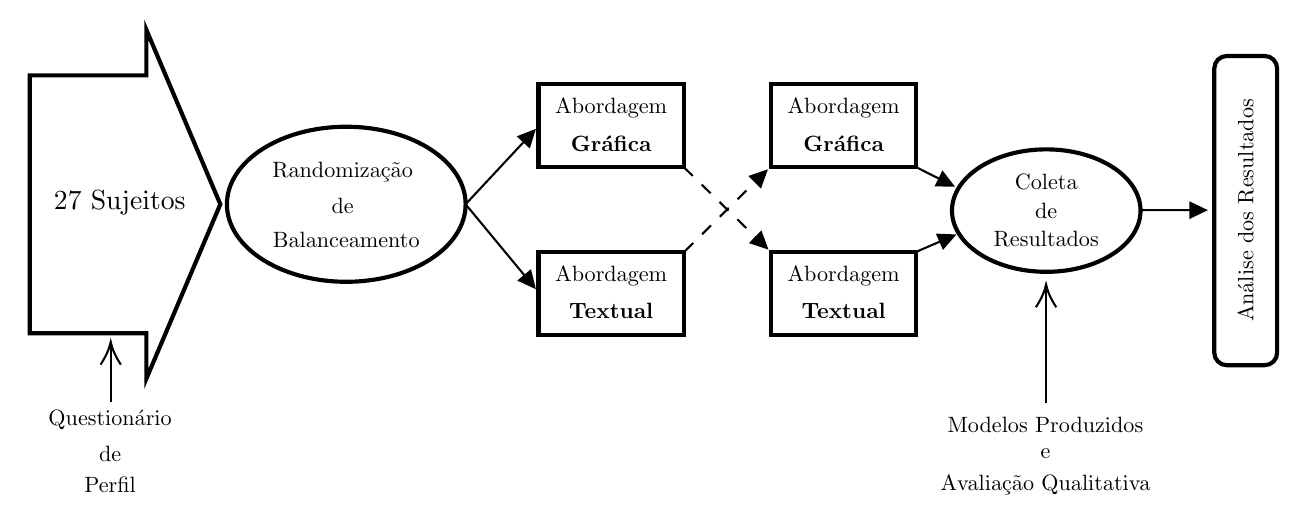
\begin{tikzpicture}[x=0.75pt,y=0.75pt,yscale=-1,xscale=1]
%uncomment if require: \path (0,327.1999969482422); %set diagram left start at 0, and has height of 327.1999969482422




%Shape: Ellipse [id:dp6331487904311781] 
\draw  [line width=1.5]  (448.63,88.9) .. controls (448.63,72.61) and (468.97,59.4) .. (494.05,59.4) .. controls (519.13,59.4) and (539.46,72.61) .. (539.46,88.9) .. controls (539.46,105.19) and (519.13,118.4) .. (494.05,118.4) .. controls (468.97,118.4) and (448.63,105.19) .. (448.63,88.9) -- cycle ;


%Shape: Rectangle [id:dp03801896284105699] 
\draw  [line width=1.5]  (249.43,28) -- (319.43,28) -- (319.43,68) -- (249.43,68) -- cycle ;

%Shape: Ellipse [id:dp583213096835353] 
\draw  [line width=1.5]  (99.3,85.85) .. controls (99.3,65.22) and (125.04,48.5) .. (156.8,48.5) .. controls (188.56,48.5) and (214.3,65.22) .. (214.3,85.85) .. controls (214.3,106.48) and (188.56,123.2) .. (156.8,123.2) .. controls (125.04,123.2) and (99.3,106.48) .. (99.3,85.85) -- cycle ;

%Straight Lines [id:da1799424135415575] 
\draw    (214.3,85.85) -- (246.81,50.98) ;
\draw [shift={(248.17,49.52)}, rotate = 493] [fill={rgb, 255:red, 0; green, 0; blue, 0 }  ][line width=0.75]  [draw opacity=0] (8.93,-4.29) -- (0,0) -- (8.93,4.29) -- cycle    ;

%Straight Lines [id:da17029537209985257] 
\draw    (214.3,85.85) -- (246.9,125.23) ;
\draw [shift={(248.17,126.77)}, rotate = 230.38] [fill={rgb, 255:red, 0; green, 0; blue, 0 }  ][line width=0.75]  [draw opacity=0] (8.93,-4.29) -- (0,0) -- (8.93,4.29) -- cycle    ;

%Straight Lines [id:da39402523544663426] 
\draw  [dash pattern={on 4.5pt off 4.5pt}]  (319.71,108.71) -- (358.51,70.41) ;
\draw [shift={(359.93,69)}, rotate = 495.36] [fill={rgb, 255:red, 0; green, 0; blue, 0 }  ][line width=0.75]  [draw opacity=0] (8.93,-4.29) -- (0,0) -- (8.93,4.29) -- cycle    ;

%Straight Lines [id:da7992081880522388] 
\draw  [dash pattern={on 4.5pt off 4.5pt}]  (319.43,68) -- (358.78,106.32) ;
\draw [shift={(360.21,107.71)}, rotate = 224.24] [fill={rgb, 255:red, 0; green, 0; blue, 0 }  ][line width=0.75]  [draw opacity=0] (8.93,-4.29) -- (0,0) -- (8.93,4.29) -- cycle    ;

%Right Arrow [id:dp4964522106990972] 
\draw  [line width=1.5]  (4.3,23.74) -- (60.47,23.74) -- (60.47,1.77) -- (96.12,85.85) -- (60.47,169.92) -- (60.47,147.96) -- (4.3,147.96) -- cycle ;

%Shape: Rectangle [id:dp003852149638719382] 
\draw  [line width=1.5]  (361.43,28) -- (431.43,28) -- (431.43,68) -- (361.43,68) -- cycle ;

%Shape: Rectangle [id:dp0126542660109914] 
\draw  [line width=1.5]  (361.43,108.75) -- (431.43,108.75) -- (431.43,148.75) -- (361.43,148.75) -- cycle ;

%Shape: Rectangle [id:dp4954877903085966] 
\draw  [line width=1.5]  (249.43,108.75) -- (319.43,108.75) -- (319.43,148.75) -- (249.43,148.75) -- cycle ;
%Straight Lines [id:da3442884963113835] 
\draw    (431.43,68) -- (448.31,76.5) ;
\draw [shift={(450.1,77.4)}, rotate = 206.72] [fill={rgb, 255:red, 0; green, 0; blue, 0 }  ][line width=0.75]  [draw opacity=0] (8.93,-4.29) -- (0,0) -- (8.93,4.29) -- cycle    ;

%Straight Lines [id:da6883068419855551] 
\draw    (431.43,108.75) -- (448.93,101.19) ;
\draw [shift={(450.77,100.4)}, rotate = 516.65] [fill={rgb, 255:red, 0; green, 0; blue, 0 }  ][line width=0.75]  [draw opacity=0] (8.93,-4.29) -- (0,0) -- (8.93,4.29) -- cycle    ;

%Rounded Rect [id:dp5928061300931144] 
\draw  [line width=1.5]  (575,20.46) .. controls (575,17.11) and (577.71,14.4) .. (581.06,14.4) -- (599.24,14.4) .. controls (602.59,14.4) and (605.3,17.11) .. (605.3,20.46) -- (605.3,157.34) .. controls (605.3,160.69) and (602.59,163.4) .. (599.24,163.4) -- (581.06,163.4) .. controls (577.71,163.4) and (575,160.69) .. (575,157.34) -- cycle ;

%Straight Lines [id:da6932528701926595] 
\draw    (539.46,88.7) -- (569.92,88.68) ;
\draw [shift={(571.92,88.68)}, rotate = 539.96] [fill={rgb, 255:red, 0; green, 0; blue, 0 }  ][line width=0.75]  [draw opacity=0] (8.93,-4.29) -- (0,0) -- (8.93,4.29) -- cycle    ;

%Straight Lines [id:da7950818392289087] 
\draw    (43.3,181.2) -- (43.3,154.2) ;
\draw [shift={(43.3,152.2)}, rotate = 450] [color={rgb, 255:red, 0; green, 0; blue, 0 }  ][line width=0.75]    (10.93,-4.9) .. controls (6.95,-2.3) and (3.31,-0.67) .. (0,0) .. controls (3.31,0.67) and (6.95,2.3) .. (10.93,4.9)   ;

%Straight Lines [id:da5784112946450906] 
\draw    (493.97,181.53) -- (493.97,126.53) ;
\draw [shift={(493.97,124.53)}, rotate = 450] [color={rgb, 255:red, 0; green, 0; blue, 0 }  ][line width=0.75]    (10.93,-4.9) .. controls (6.95,-2.3) and (3.31,-0.67) .. (0,0) .. controls (3.31,0.67) and (6.95,2.3) .. (10.93,4.9)   ;


% Text Node
\draw (47.67,85) node  [align=left] {27 Sujeitos};
% Text Node
\draw (156.8,70) node [scale=0.8] [align=left] {Randomização };
% Text Node
\draw (156.8,86.5) node [scale=0.8] [align=left] {de };
% Text Node
\draw (156.8,103) node [scale=0.8] [align=left] {Balanceamento};
% Text Node
\draw (284.43,56.5) node [scale=0.8] [align=left] {\textbf{Gráfica}};
% Text Node
\draw (284.43,39.5) node [scale=0.8] [align=left] {Abordagem};
% Text Node
\draw (396.43,39.5) node [scale=0.8] [align=left] {Abordagem};
% Text Node
\draw (396.43,56.5) node [scale=0.8] [align=left] {\textbf{Gráfica}};
% Text Node
\draw (396.43,120.25) node [scale=0.8] [align=left] {Abordagem};
% Text Node
\draw (396.43,137.25) node [scale=0.8] [align=left] {\textbf{Textual}};
% Text Node
\draw (284.43,120.25) node [scale=0.8] [align=left] {Abordagem};
% Text Node
\draw (284.43,137.25) node [scale=0.8] [align=left] {\textbf{Textual}};
% Text Node
\draw (494.05,75.15) node [scale=0.8] [align=left] {Coleta};
% Text Node
\draw (494.05,88.9) node [scale=0.8] [align=left] {de};
% Text Node
\draw (494.05,102.65) node [scale=0.8] [align=left] {Resultados};
% Text Node
\draw (590.15,88.9) node [scale=0.8,rotate=-270] [align=left] {Análise dos Resultados};
% Text Node
\draw (43,190) node [scale=0.8] [align=left] {Questionário};
% Text Node
\draw (43,206) node [scale=0.8] [align=left] {de};
% Text Node
\draw (43,221) node [scale=0.8] [align=left] {Perfil};
% Text Node
\draw (493.67,221) node [scale=0.8] [align=left] {Avaliação Qualitativa};
% Text Node
\draw (493.67,206) node [scale=0.8] [align=left] {e};
% Text Node
\draw (493.67,192) node [scale=0.8] [align=left] {Modelos Produzidos};


\end{tikzpicture}

    \fonte{Adaptado de \citeonline{Bernardino:2016}.}
\end{figure}



\subsection{Instrumentação} \label{ssec:instExp}

Como a participação no experimento foi voluntária, preparou-se um \ac{TCLE} aos participantes para o registro da concordância de todos os sujeitos na execução das atividades, apresentado no Apêndice \ref{ap:TermoExp}.
O questionário de perfil criado e aplicado para o balanceamento dos grupos e está presente no Apêndice \ref{ap:QuestPerfilExp}.
Também foi elaborado um glossário para conceitos que foram utilizados na apresentação de abertura do experimento e durante os treinamentos, exposto no Apêndice \ref{ap:GlossarioExp}.

Com a finalidade de fornecer o suporte aos participantes da avaliação, foram providenciados instrumentos descrevendo o passo a passo com exemplos, exibidos nos Apêndices \ref{ap:StepBrModeloExp} e \ref{ap:StepERDSLExp}, para o uso das ferramentas utilizadas no experimento (BrModelo e ERText). 
Além disso, foi realizado um treinamento que incluía vídeos com tutoriais de uso das abordagens em cada ferramenta. 
Os vídeos demostravam como se deveria iniciar a modelagem, exemplos dos construtores previstos nos problemas que eles teriam que resolver e as recomendações para o salvamento dos artefatos produzidos. 

Foram elaborados dois (2) instrumentos que continham um problema cada, com níveis similares de complexidade, os quais deveriam ser modelados e também anotados os horários de começo e término da atividade. 
Estes instrumentos estão nos Apêndices \ref{ap:Inst1Exp} e \ref{ap:Inst2Exp}. 
Para a posterior avaliação por parte dos sujeitos foram criados outros dois (2) instrumentos. 
O primeiro apresentava sete (7) atributos de qualidade com base na ISO/IEC 25010\footnote{https://www.iso.org/standard/35733.html}, uma norma para qualidade de produtos de software, e serviu para avaliar as abordagens das duas ferramentas do ponto de vista dos sujeitos que executaram as atividades de modelagem \ac{ER}.
Este instrumento é apresentado no Apêndice \ref{ap:Inst3Exp}.
O segundo instrumento serviu para a avaliação da representação dos construtores da solução proposta neste estudo, e está disposto no Apêndice \ref{ap:Inst4Exp}. 
Os dados gerados por estes instrumentos serviram para responder as \acp{QP} qualitativas definidas para este experimento.

Ademais, foi também gerado um ambiente de trabalho igual para todos os sujeitos do experimento. 
Para tanto, criou-se uma máquina virtual que utilizava o sistema operacional Xubuntu\footnote{https://xubuntu.org/}, uma distribuição Linux derivada do Ubuntu que utiliza o ambiente gráfico XFCE. 
Neste ambiente foram disponibilizados os materiais de apoio citados anteriormente, bem como as ferramentas de modelagem \ac{ER}. 
Para evitar possíveis influências externas as máquinas virtuais não tinham acesso com a Internet, garantindo assim que os sujeitos não poderiam realizar consultas à conteúdos externos. 
Dessa forma, foi possível assegurar que todos os sujeitos realizaram as mesmas tarefas, e nas mesmas condições.

\subsection{Ameaças à Validade} \label{ssec:validadeExp}

Objetivando que a avaliação tenha um resultado válido para o experimento proposto, foi necessário analisar e discutir as ameaças à validade, bem como as estratégias utilizadas para mitigá-las.
Para a listagem das possíveis ameaças foram utilizadas os tópicos e recomendações levantadas no trabalho de \citeonline{Wohlin:2012}. 
Essas ameaças seguiram o padrão proposto e foram divididas em quatro (4) categorias, sendo: validade do construto, validade interna, validade externa e validade de conclusão.

\subsubsection{Validade do Construto}

A validade do construto diz respeito ao \textit{design} do experimento e a fatores sociais.

\textit{\textbf{Explicação pré-operacional inadequada}}: Esta ameaça está relacionada com o fato do experimento não ter o objetivo dos artefatos suficientemente definidos antes de serem traduzidos em medidas ou tratamentos. 
Para mitigar essa ameaça foi comparado o esforço em tempo de cada abordagem, bem como foi realizada a verificação da efetividade de acordo com os conceitos de \textit{Precisão} e \textit{Revocação} da \textit{Medida-F}.

\textit{\textbf{Interação de diferentes tratamentos}}. Se os sujeitos estiverem envolvidos em mais de um estudo, os tratamentos dos diferentes estudos poderão interagir e reverberar nos resultados finais. 
Como este experimento seguiu um \textit{design} pareado, todos os sujeitos realizaram os dois tratamentos. 
Contudo, não foi identificado aprendizado entre a execução das atividades.
Isto pode ser verificado por meio da normalidade das distribuições analisadas das amostras de esforço e efetividade, as quais demonstram que os resultados mantiveram-se semelhantes como um todo.

\textit{\textbf{Predição das hipóteses}}: 
Quando os sujeitos participam de um experimento é possível que tentem descobrir qual é o objetivo ou o resultado pretendido do experimento. 
Este fato pode trazer viés ao comportamento, positivamente ou negativamente, dependendo da hipótese antecipada.
Para mitigar essa ameaça os sujeitos não foram informados sobre maiores detalhes do experimento \textit{e.g.} perguntas de pesquisa, hipóteses, objetivos e propósito.


\subsubsection{Validade Interna}

Ameaças à validade interna são influências que podem afetar as variáveis independentes em relação à causalidade, sem o conhecimento do pesquisador. 

\textit{\textbf{História}}: Há o risco de algum período temporal específico ter influência na realização do experimento. 
Para mitigar esta ameaça, e em razão do experimento ser realizado em ambiente acadêmico, todo o processo foi executado no mês de agosto, em que no geral os alunos não estão necessariamente sobrecarregados com atividades acadêmicas \textit{e.g.} provas e trabalhos.

\textit{\textbf{Maturação}}: Essa é a ameaça que ocorre em relação aos sujeitos reagirem de maneiras diferentes com o passar do tempo. 
Exemplos são quando os sujeitos são afetados negativamente (cansaço ou tédio) ou positivamente (aprendizado) durante o curso do experimento.
Para mitigar essa ameaça foi comunicado desde o início aos sujeitos que poderiam encerrar a sua participação no momento que quisessem, sem qualquer tipo de penalização.

\textit{\textbf{Testes}}: Se os testes forem repetidos, os sujeitos podem responder de maneira diferente em momentos diferentes, pois sabem como o teste é realizado. 
Se houver necessidade de familiarização com os testes, é importante que os resultados do teste não sejam devolvidos ao sujeito, para assim não apoiar o aprendizado não intencional. 
Não houve necessidade de repetição das atividades, uma vez que as mesmas foram executadas uma vez por participante em cada tratamento.

\textit{\textbf{Instrumentação}}: Essa ameaça está relacionada aos artefatos usados para a execução da experiência, como formulários de coleta de dados, etc.
Se estes foram mal projetados, a experiência é afetada negativamente.
Para combater essa ameaça, todos os artefatos foram verificados e validados previamente em reuniões entre os pesquisadores envolvidos neste trabalho.
Além disso, foi realizado um estudo piloto para validar o protocolo planejado para o experimento.

\subsubsection{Validade Externa}

As ameaças à validade externa são as condições relacionadas a replicação do experimento.

\textit{\textbf{Sujeitos do experimento}}: Os sujeitos selecionados para o experimento podem não representar um grupo significativo para a área de estudo. 
Buscando tentar mitigar essa ameaça o experimento foi realizado com estudantes de Engenharia de Software e Ciência da Computação, e logo, inseridos no contexto de uso da modelagem conceitual de \acp{BD} relacionais.
Porém, o fato da amostra ter menos de trita (30) elementos é uma ameaça estatística na área analisada, e não foi possível mitigar este fato.

\textit{\textbf{Interação dos sujeitos com os artefatos de avaliação}}: Essa é a ameaça relacionada a aplicação dos artefatos de avaliação do experimento com os sujeitos.
Dependendo do momento isto pode afetar os resultados.
Se, por exemplo, um questionário for realizado alguns dias após a execução do experimento, as pessoas tendem a responder de maneira diferente do que fariam momentos após as atividades.

\textit{\textbf{Interação de configuração e tratamento}}: São ameaças relacionadas ao fato de se usar uma configuração ou material não representativo. 
Para mitigar essa ameaça, foi utilizada uma documentação com base em \textit{templates} e modelos tradicionais encontrados em material de ensino de \acp{BD}. 
Além disso, os artefatos foram validados com dois especialistas da área de Engenharia de Software.

Um ponto importante quanto a validade externa é que as ameaças podem ser reduzidas tornando o ambiente experimental o mais realista possível. 
Por outro lado, a realidade nem sempre é homogênea. 
Porém,  mais importante é definir e relatar as características do ambiente, como experiência da equipe, ferramentas, métodos de avaliação e a aplicabilidade em um contexto específico \cite{Wohlin:2012}.

\subsubsection{Validade da Conclusão}

As ameaças à validade da conclusão estão relacionadas com questões que afetam a capacidade de se inferir uma conclusão correta sobre as relações entre os tratamentos e o resultado de um experimento.

\textit{\textbf{Baixo poder estatístico}}: Uma possível ameaça nesta categoria é o baixo poder estatístico.
Para tentar mitigar esta ameaça foi adotado alguns métodos estatísticos como o teste de normalidade Shapiro-Wilk, o Teste T pareado como teste de hipótese para amostras dependentes, e a Medida-F para análise qualitativa dos modelos produzidos.

\textit{\textbf{Confiabilidade das medições}}: A confiabilidade das medições utilizadas tem impacto direto na validade do experimento como um todo. Para mitigar essa ameaça foram realizadas medições objetivas que não dependiam de julgamento subjetivo (esforço, medido em tempo, e Medida-F). 
Por outro lado, as métricas utilizadas para a avaliação qualitativa ainda serviram como insumo complementar na discussão dos resultados obtidos.

\textit{\textbf{Ambiente experimental}}: O experimento deve ser realizado em um ambiente controlado, procurando evitar influẽncias externas. Para mitigar esta possível ameaça os
participantes foram orientados que não poderia ocorrer conversas durante todo o tempo das atividades, nem saídas do ambiente ou acesso a dispositivos eletrônicos.


%#################################################################
\section{Operação do Experimento} \label{ssec:operacaoExp}
%#################################################################

A operação do experimento pode ser dividida em duas (2) etapas: preparação e execução.
Esta seção descreve de forma geral as ações realizadas em ambas as etapas.

%#################################################################
\subsection{Preparação}
%#################################################################

Inicialmente ocorreram reuniões entre os pesquisadores envolvidos para definição geral do planejamento e do modo de operação que deveria ser adotado.
Buscando captar uma amostra significativa para o objeto do estudo, optou-se pelo contato com a docente responsável por ministrar as disciplinas de Banco de Dados (Engenharia de Software) e Banco de Dados I (Ciência da Computação) em 2019/2.
Após reuniões para explicar os objetivos do trabalho, houve a concordância quanto a viabilidade do experimento.
Com os objetivos iniciais alinhavados, a docente que colaborou realizou a divulgação dos questionários de perfil via plataforma Moodle para os alunos matriculados.
Com os alunos do mestrado não foi possível o envio antecipado dos questionários, e por conta disso o mesmo foi aplicado no dia do experimento.

Com as respostas daqueles que retornaram o formulário de nivelamento, tantos os alunos de Engenharia de Software quanto de Ciência da Computação, começou-se a realizar com antecedência o nivelamento dos possíveis candidatos a participar do experimento.
Após a elaboração de todos os artefatos que seriam utilizados no experimento, os mesmos foram analisados e validados em conjunto pelos pesquisadores envolvidos neste estudo, havendo ainda nesse percurso a necessidade de adequação de alguns instrumentos quanto as sugestões e eventuais correções necessárias.

%#################################################################
\subsection{Execução}
%#################################################################

No dia do experimento a primeira atividade realizada foi uma breve apresentação inicial onde era informado que o experimento era de caráter não avaliativo.
Com isto esclarecido, era então disponibilizado o \ac{TCLE} (\ref{ap:TermoExp}) para todos os participantes.
Após a assinatura do \ac{TCLE}, foram distribuídos os questionários de perfil para aqueles participantes que ainda não haviam o preenchido anteriormente.
Foi constatado que não havia fortes discrepâncias entre os níveis de conhecimento dos sujeitos, demonstrando assim que no geral era uma amostra homogênea.

Antes da divisão randômica dos grupos foi realizada então a fase de treinamento. 
Durante essa etapa foram apresentadas ambas as ferramentas que seriam utilizadas, passando uma visão geral de operação e respondendo a possíveis dúvidas que pudessem surgir.
O treinamento incluía a exibição de vídeos demonstrando as ferramentas, primeiramente do BrModelo e após do editor Eclipse com o \textit{plugin} da \ac{DSL} proposta, respectivamente, com cerca de nove (9) e onze (11) minutos. 

Então, deu-se início a fase de modelagem dos problemas propostos.
Todos os participantes receberam o Instrumento 1 (\ref{ap:Inst1Exp}) e foram informados com qual ferramenta deveriam desenvolver a solução.
Foi solicitado que cada sujeito anotasse no instrumento sua identificação e o horário de início da tarefa.
Não foi estipulado nenhum tempo limite para o término e, conforme os sujeitos finalizavam a modelagem, era pedido que cumprissem as orientações inclusas no material de apoio para o salvamento dos artefatos gerados.
Com os modelos salvos, os instrumentos eram recolhidos e passava-se para a próxima tarefa descrita no Instrumento 2 (\ref{ap:Inst2Exp}), porém sendo necessário o uso da abordagem inversa a que haviam utilizado inicialmente.

Ao término dos instrumentos que continham os problemas de modelagem, foi entregue os instrumentos de avaliação qualitativa (\ref{ap:Inst3Exp} e \ref{ap:Inst4Exp}). 
Conforme os participantes finalizavam o preenchimento da avaliação, eram então liberados.
Com a conclusão do experimento por parte dos vinte e sete (27) sujeitos, encerrou-se o experimento e partiu-se para a etapa de tabulação e análise dos resultados.

%#################################################################
\section{Resultados} \label{sec:resultExp}
%#################################################################

Esta seção relata a análise dos resultados obtidos a partir dos material coletado no experimento. 
%Com base nos dados foi possível responder as questões de pesquisa e, quando fosse o caso, as hipóteses relacionadas.
É importante salientar que toda a análise estatística foi realizada com apoio da Linguagem R\footnote{RStudio: \url{https://rstudio.com}}, bem como nas recomendações do livro referência de \citeonline{Triola:2017}.

\subsection{Esforço}

Para responder a \ac{QP}1 referente ao esforço de uso das abordagens, os tempos foram extraídos dos instrumentos. 
A \autoref{tab:TemposGeral} exibe os valores associados aos sujeitos, bem como a ordem de execução das abordagens.

\begin{table}[!htb]
    \caption{Tempos de execução de cada abordagens.}
    \label{tab:TemposGeral}
    \centering
    \tiny
    \begin{tabular}{c|cc|cc}
    \bottomrule
    \rowcolor[HTML]{C0C0C0}
    \multicolumn{1}{r}{Sujeito} &
    \multicolumn{2}{c}{\textbf{Abordagem (minutos)}} &
    \multicolumn{2}{c}{\textbf{Abordagem (minutos)}}
    \\ 
    \hline
    01	&	Gráfica	&	25	&	Textual	&	48	\\
    02	&	Gráfica	&	26	&	Textual	&	45	\\
    03	&	Gráfica	&	28	&	Textual	&	38	\\
    04	&	Gráfica	&	21	&	Textual	&	28	\\
    05	&	Gráfica	&	31	&	Textual	&	20	\\
    06	&	Gráfica	&	42	&	Textual	&	26	\\
    07	&	Gráfica	&	60	&	Textual	&	58	\\
    08	&	Gráfica	&	22	&	Textual	&	36	\\
    09	&	Gráfica	&	22	&	Textual	&	28	\\
    10	&	Gráfica	&	22	&	Textual	&	30	\\
    11	&	Gráfica	&	20	&	Textual	&	28	\\
    12	&	Gráfica	&	18	&	Textual	&	30	\\
    13	&	Gráfica	&	21	&	Textual	&	15	\\
    14	&	Gráfica	&	12	&	Textual	&	16	\\
    15	&	Textual	&	60	&	Gráfica	&	28	\\
    16	&	Textual	&	18	&	Gráfica	&	22	\\
    17	&	Textual	&	56	&	Gráfica	&	27	\\
    18	&	Textual	&	38	&	Gráfica	&	28	\\
    19	&	Textual	&	60	&	Gráfica	&	28	\\
    20	&	Textual	&	41	&	Gráfica	&	46	\\
    21	&	Textual	&	33	&	Gráfica	&	20	\\
    22	&	Textual	&	57	&	Gráfica	&	35	\\
    23	&	Textual	&	32	&	Gráfica	&	17	\\
    24	&	Textual	&	35	&	Gráfica	&	28	\\
    25	&	Textual	&	38	&	Gráfica	&	26	\\
    26	&	Textual	&	20	&	Gráfica	&	25	\\
    27	&	Textual	&	18	&	Gráfica	&	12	\\
    \toprule
    \end{tabular}
    \fonte{O autor.}
\end{table}

A partir dos valores brutos dos tempos foi calculada a diferença para ser possível realizar o teste de normalidade Shapiro-Wilk.
Por ser um teste estatístico, esta técnica tem como produto a medida do valor-$p$.
Para este teste foi adotado um nível de significância $\alpha$~=~5\%. 
Isso significa que se o valor-$p$ for menor que 5\% ($p$ < 0.05), a hipótese nula de que a distribuição é normal deve ser rejeitada.

Após os cálculos com o conjunto das diferenças dos tempos chegou-se a um valor-$p$ de 0.606530.
Como valor-$p$ > $\alpha$, a hipótese nula foi aceita, concluindo assim que os dados são normalmente distribuídos.
Em outras palavras, a diferença entre a amostra de dados e a distribuição normal não é grande o suficiente para ser estatisticamente significativa.

É importante ressaltar que quanto maior o valor-$p$, mais ele suporta uma hipótese nula. 
No caso do resultado obtido a chance de erro do tipo 1 (rejeitar uma hipótese nula que é correta) é muito alta, podendo ser traduzida em 60,65\% (0.606530).

Ainda em relação ao teste de normalidade, o valor de \textit{W} calculado foi de 0.970178, estando dentro do intervalo aceito do valor crítico de 95\% (0.9242 : 1.0000). 
Isto significa que existe 95\% de chances da amostra ter origem em uma população normal.
A \autoref{fig:DistTempo} apresenta uma representação visual da distribuição analisada.

\begin{figure}[!htb]
    \centering
    \caption{Distribuição amostral referente ao esforço.}
    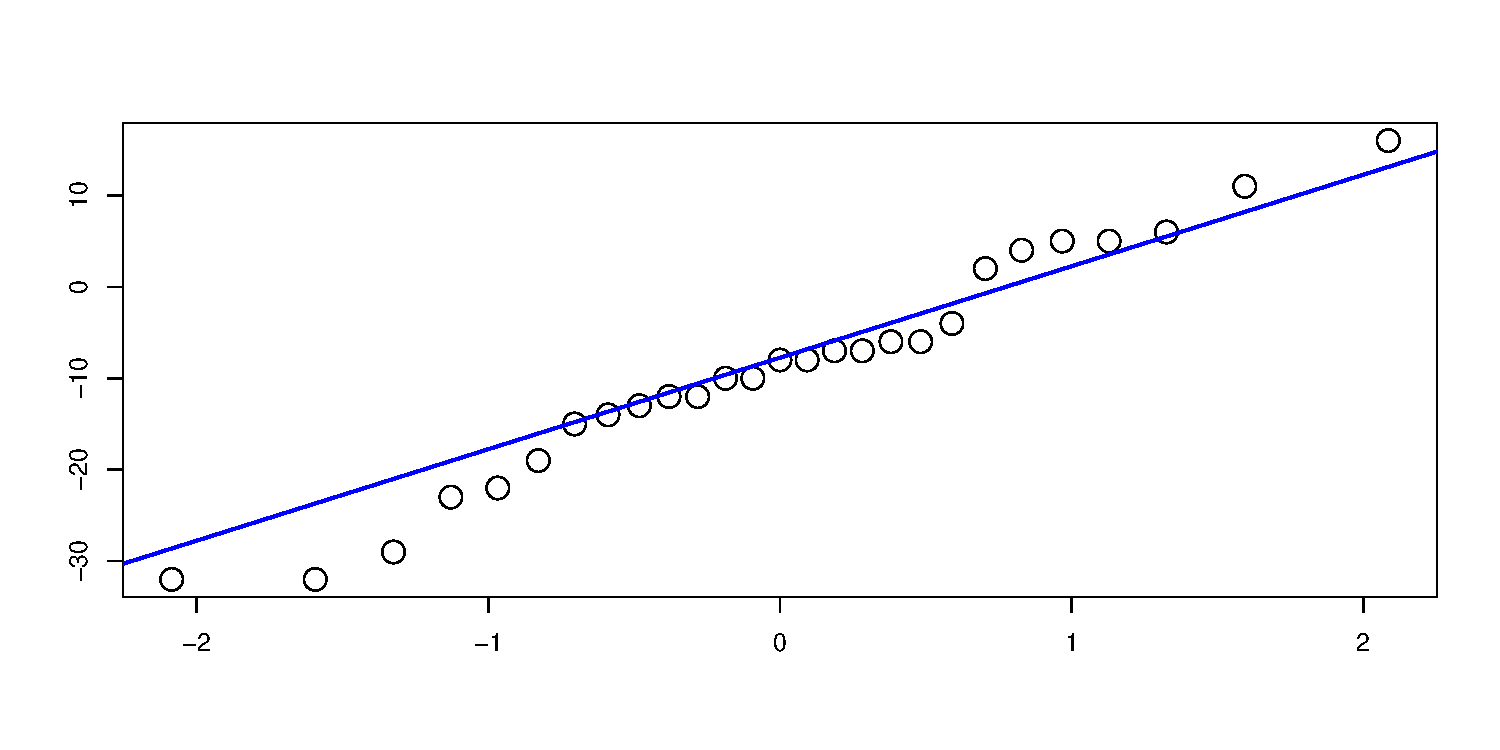
\includegraphics[width=0.7\textwidth]{ResultsExp/DistribuicaoAmostraTempo}
    \label{fig:DistTempo}
    \fonte{O autor.}
\end{figure}

Tendo sido a amostra testada quanto à sua normalidade, foi possível realizar o teste da primeira hipótese estabelecida neste experimento. 
No teste T pareado para amostras dependentes foi utilizado um nível de significância $\alpha$~=~5\%, com o qual se chegou a uma medida de 0.000962084 para o valor-$p$. 
Por ser um teste bicaudal, ou seja, que inclui uma igualdade na sua hipótese nula, esse valor-$p$ mostra evidências suficientes para garantir a rejeição da afirmativa de $H_0 : \mu Tempo_G = \mu Tempo_T$.
Logo, a hipótese alternativa de que as abordagens possuem esforços diferentes é aceita, pois segundo o teste essa diferença é estatisticamente significativa.

A \autoref{tab:TemposGeralMedidas} mostra os valores que possibilitam uma análise de dispersão. A \autoref{fig:boxplotTempo} exibe um \textit{boxplot} com a variação de dados observados por meio destes dados. 
Com base nestes dados e na sua representação visual, é possível verificar que, em média, a abordagem gráfica leva vantagem sobre a abordagem textual. 

\begin{table}[!htb]
    \caption{Medidas relacionadas ao esforço médio.}
    \label{tab:TemposGeralMedidas}
    \centering
    \footnotesize
    \begin{tabular}{l|lc|lc}
    \bottomrule
    \rowcolor[HTML]{C0C0C0}
    \multicolumn{1}{c}{\textbf{}} &
    \multicolumn{2}{c}{\textbf{Abordagem}}
    \\
    \rowcolor[HTML]{C0C0C0}
    \multicolumn{1}{c}{\textbf{Medida}} &
    \multicolumn{1}{c}{\textbf{Gráfica}} &
    \multicolumn{1}{c}{\textbf{Textual}}
    \\
    \hline
        Limite Inferior 	&	12.00   &   15.00   \\
        1\degree Quartil	&	21.00	&   27.00   \\
        Média	            &	26.37	&   35.26   \\
        Mediana	            &	25.00   &   33.00   \\
        3\degree Quartil	&	28.00   &   43.00   \\
        Limite superior	    &	60.00   &   60.00   \\
        Desvio Padrão	    &  	10.12	&	14.03	\\
    \toprule
    \end{tabular}
    \fonte{O autor.}
\end{table}


\begin{figure}[!htb]
    \centering
    \caption{Tempos medidos nos tratamentos.}
    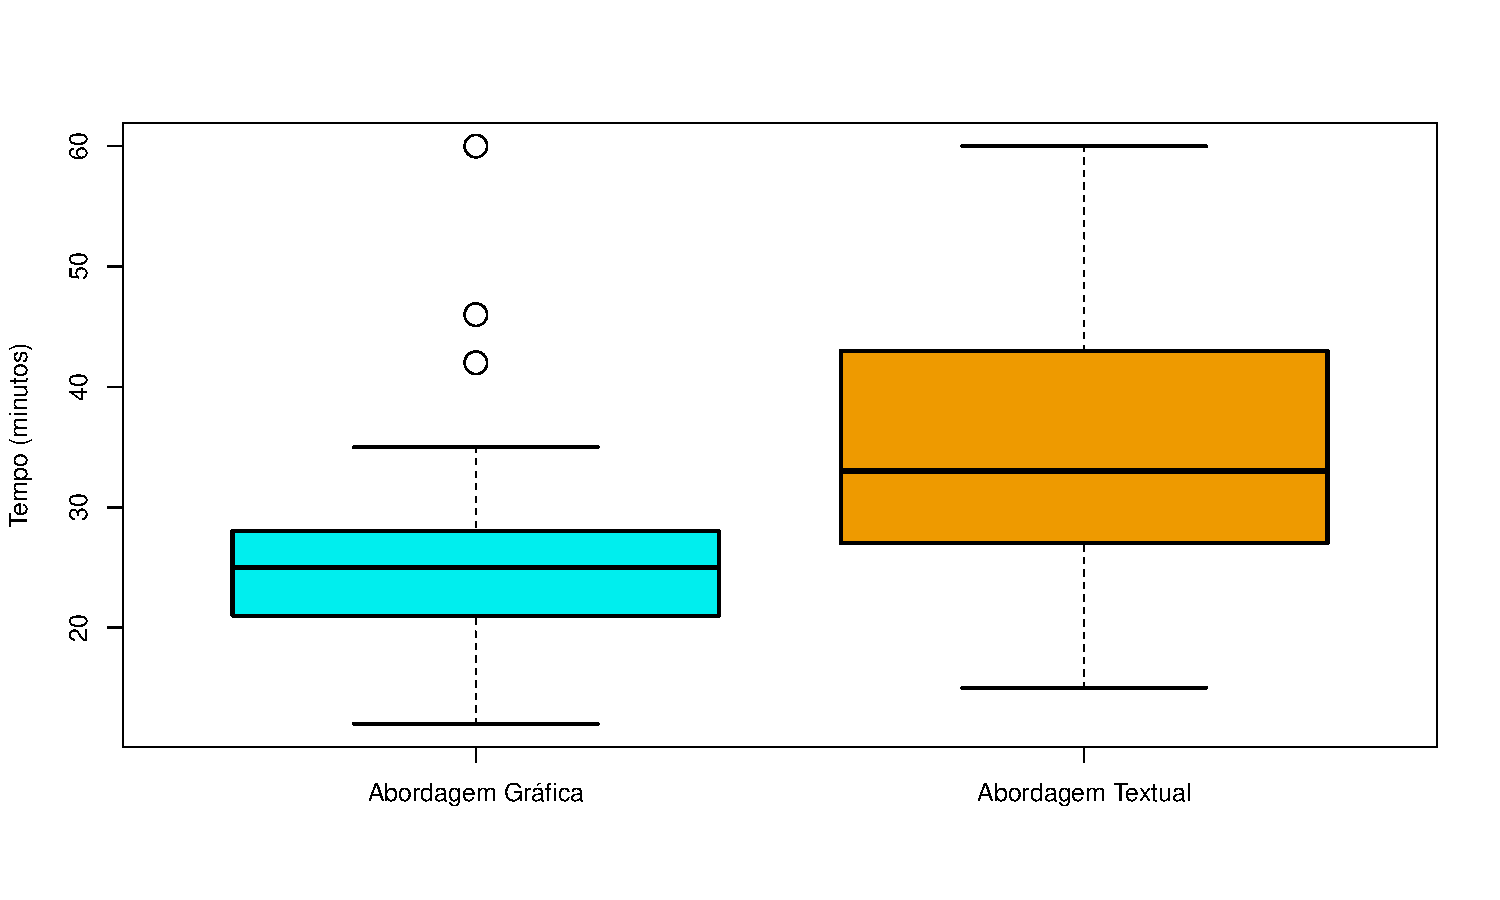
\includegraphics[width=0.8\textwidth]{ResultsExp/BoxPlotTempo}
    \label{fig:boxplotTempo}
    \fonte{O autor.}
\end{figure}



\subsection{Efetividade}
Para responder a \ac{QP}2 referente a efetividade do uso das abordagens, os artefatos produzidos pelos sujeitos foram avaliados conforme os modelos de referência estabelecidos.

\rowcolors{1}{gray!15}{white}
\begin{landscape}
\begin{table}[!htb]
    \caption{Avaliação dos modelos produzidos no experimento.}
    \label{tab:ResultsModelosIndividual}
    \centering
    \footnotesize
    
    \begin{tabular}{l|cc|ccc|cc|ccc}
    \bottomrule
    \rowcolor[HTML]{C0C0C0}
    \multicolumn{1}{l}{} &
    \multicolumn{5}{c}{\textbf{Abordagem Gráfica}} &
    \multicolumn{5}{c}{\textbf{Abordagem Textual}}
    \\ 
    \hline
    \rowcolor[HTML]{C0C0C0}
    \textbf{P} & \textbf{IM} & \textbf{IR} & \textbf{Precisão (\%)} & \textbf{Revocação (\%)} & \textbf{Medida-F (\%)} &
    \textbf{IM} & \textbf{IR} & \textbf{Precisão (\%)} & \textbf{Revocação (\%)} & \textbf{Medida-F (\%)}
    \\
    01	&	23	&	17	&	73.91	&	36.96	&	49.28	&	29	&	24	&	82.76	&	60.00	&	69.57	\\
    02	&	41	&	33	&	80.49	&	84.62	&	82.50	&	67	&	41	&	61.19	&	87.23	&	71.93	\\
    03	&	38	&	28	&	73.68	&	71.79	&	72.73	&	50	&	42	&	84.00	&	89.36	&	86.60	\\
    04	&	36	&	25	&	69.44	&	64.10	&	66.67	&	44	&	32	&	72.73	&	68.09	&	70.33	\\
    05	&	32	&	26	&	81.25	&	66.67	&	73.24	&	31	&	28	&	90.32	&	59.57	&	71.79	\\
    06	&	32	&	24	&	75.00	&	61.54	&	67.61	&	38	&	36	&	94.74	&	76.60	&	84.71	\\
    07	&	37	&	32	&	86.49	&	69.57	&	77.11	&	23	&	21	&	91.30	&	52.50	&	66.67	\\
    08	&	41	&	34	&	82.93	&	87.18	&	85.00	&	44	&	39	&	88.64	&	97.50	&	92.86	\\
    09	&	36	&	31	&	86.11	&	79.49	&	82.67	&	36	&	30	&	83.33	&	63.83	&	72.29	\\
    10	&	38	&	33	&	86.84	&	84.62	&	85.71	&	20	&	19	&	95.00	&	40.43	&	56.72	\\
    11	&	40	&	35	&	87.50	&	76.09	&	81.40	&	29	&	25	&	86.21	&	62.50	&	72.46	\\
    12	&	53	&	33	&	62.26	&	84.62	&	71.74	&	53	&	42	&	79.25	&	89.36	&	84.00	\\
    13	&	37	&	34	&	91.89	&	73.91	&	81.93	&	48	&	35	&	72.92	&	87.50	&	79.55	\\
    14	&	46	&	33	&	71.74	&	84.62	&	77.65	&	36	&	29	&	80.56	&	61.70	&	69.88	\\
    15	&	29	&	27	&	93.10	&	69.23	&	79.41	&	41	&	37	&	90.24	&	78.72	&	84.09	\\
    16	&	33	&	25	&	75.76	&	54.35	&	63.29	&	34	&	30	&	88.24	&	75.00	&	81.08	\\
    17	&	39	&	26	&	66.67	&	66.67	&	66.67	&	45	&	37	&	82.22	&	78.72	&	80.43	\\
    18	&	40	&	35	&	87.50	&	89.74	&	88.61	&	45	&	43	&	95.56	&	91.49	&	93.48	\\
    19	&	27	&	24	&	88.89	&	52.17	&	65.75	&	51	&	32	&	62.75	&	80.00	&	70.33	\\
    20	&	25	&	24	&	96.00	&	52.17	&	67.61	&	34	&	25	&	73.53	&	62.50	&	67.57	\\
    21	&	36	&	33	&	91.67	&	71.74	&	80.49	&	35	&	30	&	85.71	&	75.00	&	80.00	\\
    22	&	34	&	29	&	85.29	&	74.36	&	79.45	&	44	&	38	&	86.36	&	80.85	&	83.52	\\
    23	&	42	&	32	&	76.19	&	82.05	&	79.01	&	41	&	27	&	65.85	&	57.45	&	61.36	\\
    24	&	28	&	19	&	67.86	&	41.30	&	51.35	&	26	&	19	&	73.08	&	47.50	&	57.58	\\
    25	&	36	&	32	&	88.89	&	82.05	&	85.33	&	38	&	35	&	92.11	&	74.47	&	82.35	\\
    26	&	34	&	13	&	38.24	&	33.33	&	35.62	&	31	&	18	&	58.06	&	38.30	&	46.15	\\
    27	&	31	&	26	&	83.87	&	56.52	&	67.53	&	37	&	31	&	83.78	&	77.50	&	80.52	\\
    \toprule
    \end{tabular}
    \begin{tablenotes}
    \tiny
    \item Legenda: IM (\textit{Itens Modelados}) IR (\textit{Itens Relevantes})
    \end{tablenotes}
    \fonte{O autor.}
\end{table}
\end{landscape}

Nesta avaliação foi utilizada a Medida-F, uma medida proveniente da área de reconhecimento de padrões e recuperação de informação. 
A Medida-F representa a combinação da precisão e revocabilidade observada de um resultado em relação à uma referência.

Por definição, essa combinação se refere à fração de instâncias recuperadas que são relevantes (precisão) e a fração de instâncias relevantes que são recuperadas  (revocabilidade).
A \autoref{tab:ResultsModelosIndividual} exibe estes valores associados obtidos pelos sujeitos, separados pelos tratamentos realizados.

Após a obtenção dos valores da Medida-F de cada modelo, foi realizado o teste de normalidade Shapiro-Wilk.
Após os cálculos com o conjunto das diferenças da Medida-F de cada modelo, chegou-se a um valor-$p$ de 0.404455.
Com este resultado obtido a chance de erro do tipo 1 (rejeitar uma hipótese nula que é correta) pode ser muito alta, podendo ser traduzida em 40,45\% (0.404455).

Como o valor-$p$ > $\alpha$, a hipótese nula foi aceita, constatando assim que os dados são normalmente distribuídos, isto é, a diferença entre a amostra de dados e a distribuição normal não é grande o suficiente para ser estatisticamente significativa.
A \autoref{fig:distMedidaF} apresenta a representação visual da distribuição do conjunto de diferenças da Medida-F dos modelos.

\begin{figure}[!htb]
    \centering
    \caption{Distribuição amostral referente a efetividade.}
    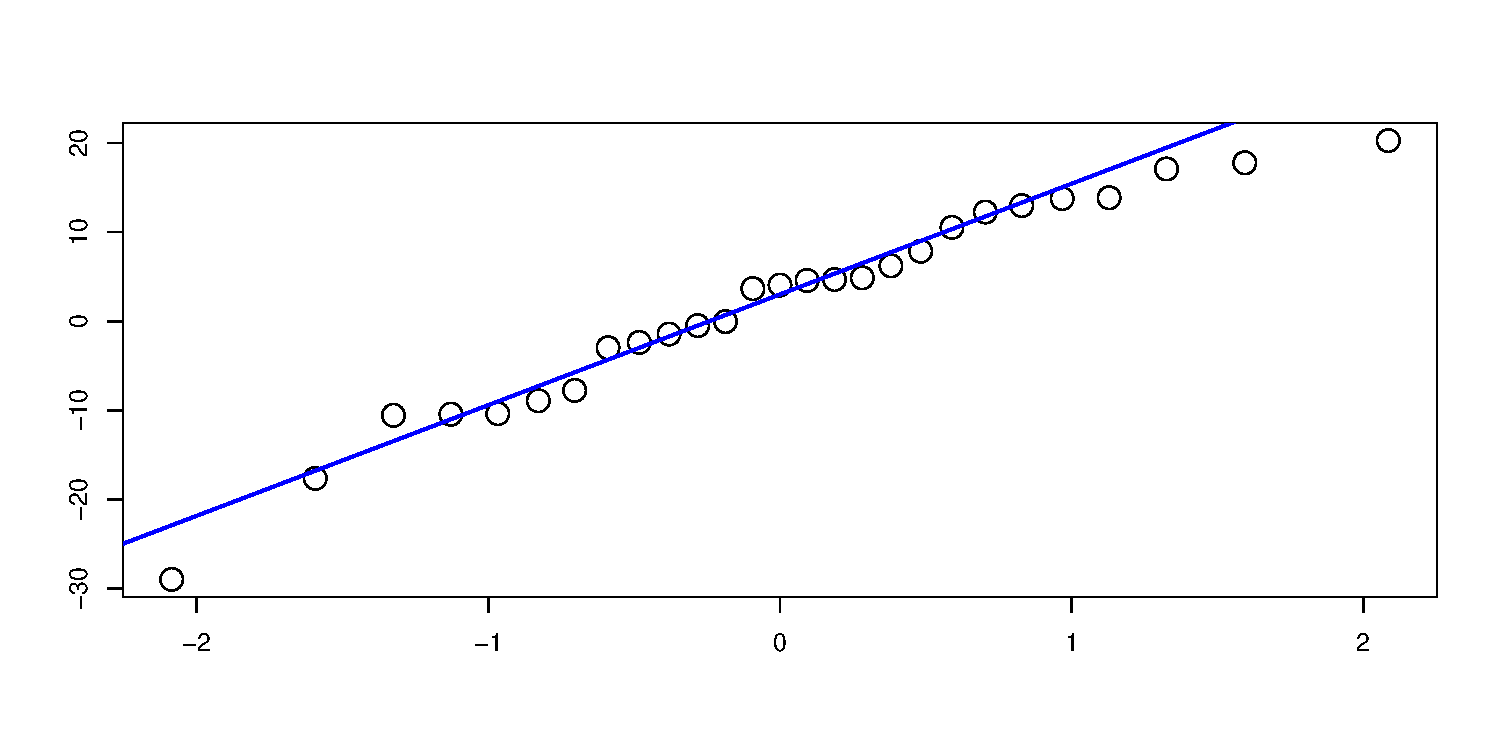
\includegraphics[width=0.7\textwidth]{ResultsExp/DistribuicaoAmostraFScore}
    \label{fig:distMedidaF}
    \fonte{O autor.}
\end{figure}

Após a amostra ser testada quanto à sua normalidade, foi realizado o teste da segunda hipótese definida neste experimento. 
Desta vez, no teste T pareado para amostra dependentes, novamente foi utilizado um nível de significância $\alpha$~=~5\%, com o qual se chegou a uma medida de 0.396468 para o valor-$p$. 

Pela afirmativa original incluir uma igualdade, caracterizando também este teste como bicaudal, chegou-se a conclusão que o valor-$p$ calculado demonstra que não há evidências suficientes para garantir a rejeição da afirmativa da hipótese nula original, denotada como $H_0 : \mu Efetividade_G = \mu Efetividade_T$.
Logo, a hipótese nula de que as abordagens possuem efetividades iguais é aceita, pois segundo o teste a diferença média da Medida-F entre os tratamentos não é estatisticamente significativa.

A \autoref{tab:ResultsModelosGeral} mostra medidas médias dos valores avaliados, e também fornecem a possibilidade para a realização de uma análise de dispersão. 


\begin{table}[!htb]
    \caption{Médias gerais da avaliação dos modelos produzidos no experimento.}
    \label{tab:ResultsModelosGeral}
    \centering
    \tiny
    
    \begin{tabular}{l|cc|ccc|cc|ccc}
    \bottomrule
    \rowcolor[HTML]{C0C0C0}
    \multicolumn{1}{l}{} &
    \multicolumn{5}{c}{\textbf{Abordagem Gráfica}} &
    \multicolumn{5}{c}{\textbf{Abordagem Textual}}
    \\ 
    \hline
    \rowcolor[HTML]{C0C0C0}
    Medida & \textbf{IM} & \textbf{IR} & \textbf{P (\%)} & \textbf{R (\%)} & \textbf{MF (\%)} &
    \textbf{IM} & \textbf{IR} & \textbf{P (\%)} & \textbf{R (\%)} & \textbf{MF (\%)}
    \\
Limite Inferior	&	23.00	&	13.00	&	38.24	&	33.33	&	35.62	&	20.00	&	18.00	&	58.06	&	38.30	&	46.15	\\
1\degree Quartil	&	32.00	&	25.00	&	73.80	&	59.03	&	67.10	&	32.50	&	26.00	&	73.30	&	60.85	&	69.72	\\
Média	&	35.70	&	28.26	&	79.61	&	68.57	&	72.79	&	38.89	&	31.30	&	81.50	&	70.88	&	74.73	\\
Mediana	&	36.00	&	29.00	&	82.93	&	71.74	&	77.11	&	38.00	&	31.00	&	83.78	&	75.00	&	72.46	\\
3\degree Quartil	&	39.50	&	33.00	&	87.50	&	82.05	&	81.66	&	44.50	&	37.00	&	89.44	&	80.43	&	82.93	\\
Limite Superior	&	53.00	&	35.00	&	96.00	&	89.74	&	88.61	&	67.00	&	43.00	&	95.56	&	97.50	&	93.48	\\
Desvio Padrão	&	6.33	&	5.63	&	11.94	&	15.39	&	12.16	&	9.97	&	7.30	&	10.44	&	15.36	&	10.94	\\
 \toprule
    \end{tabular}
    \begin{tablenotes}
    \tiny
    \item Legenda: IM (\textit{Itens Modelados}) IR (\textit{Itens Relevantes})
    P (\textit{Precisão}) R (\textit{Revocação})
    MF (\textit{Medida-F})
    \end{tablenotes}
    \fonte{O autor.}
\end{table}

O \textit{boxplot} da \autoref{fig:BoxPlotMedidaF} exibe uma representação visual da Medida-F dos tratamentos aplicados.
Com base neste gráfico é possível verificar o resultado obtido no teste de hipótese pois a dispersão dos dados não apresenta grande diferença entre as abordagens. 

\begin{figure}[!htb]
    \centering
    \caption{\textit{Boxplot} da Medida-F dos tratamentos.}
    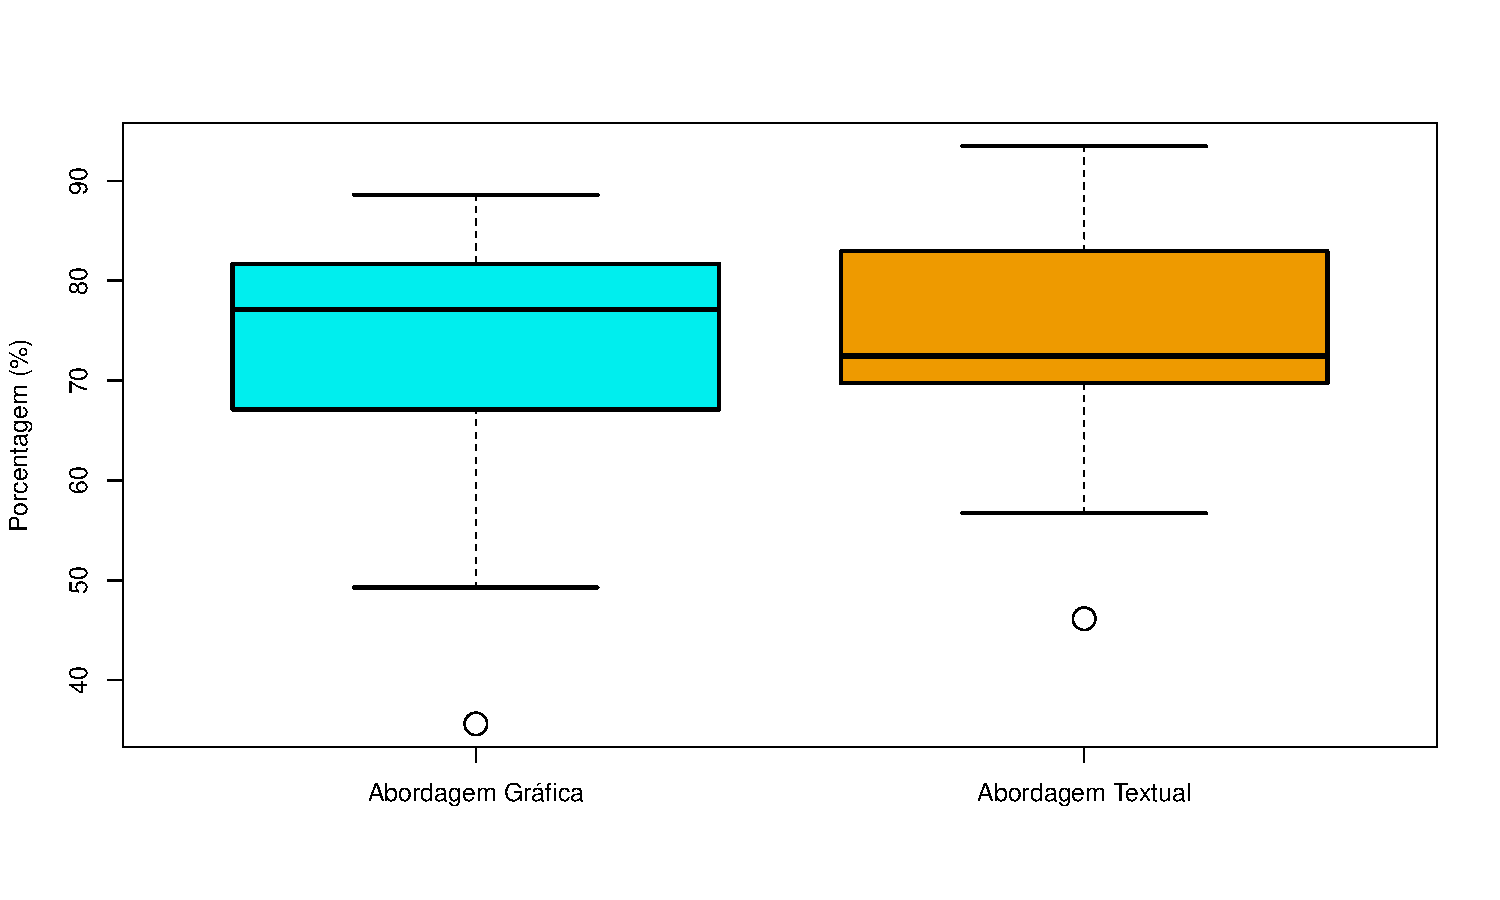
\includegraphics[width=0.8\textwidth]{ResultsExp/BoxPlotAcertos}
    \label{fig:BoxPlotMedidaF}
    \fonte{O autor.}
\end{figure}

% \begin{figure}[!htb]
%     \centering
%     \caption{Boxplot da \textit{Precisão} e \textit{Revocação} medidos nas abordagens.}
%     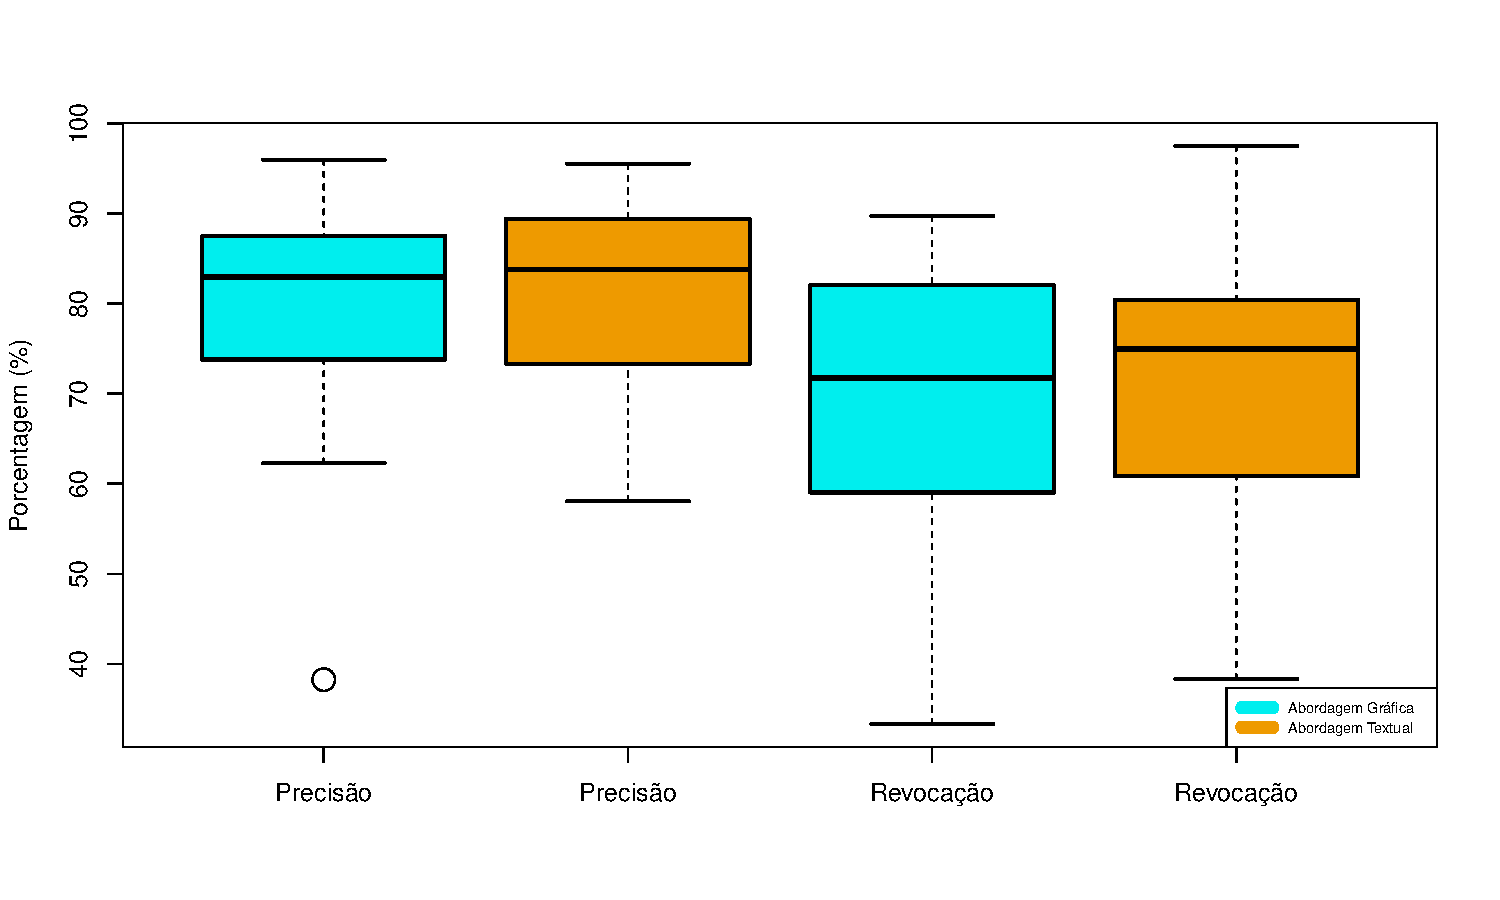
\includegraphics[width=0.7\textwidth]{ResultsExp/PrecisaoRevocacao}
%     \label{fig:BoxPlotPrecisaoRevocacao}
%     \fonte{O autor.}
% \end{figure}

\subsection{Avaliação Qualitativa}


A avaliação qualitativa se deu com a análise dos instrumentos aplicados após as tarefas de modelagem.
O primeiro destes, presente no Apêndice \ref{ap:Inst3Exp}, foi utilizado para responder a \ac{QP}3 referente a percepção de utilidade e facilidade de uso dos tratamentos.
Isto ocorreu mediante a seleção de atributos de qualidade descritos na ISO/IEC 25010.

Para tanto, foi estabelecido uma escala Likert de um (1) até seis (6).
Esta escala serviu para medir o nível de concordância dos sujeitos perante as afirmativas expostas no formulário.
Optou-se por um número par de alternativas para evitar possíveis respostas neutras.
Os sete (7) atributos de qualidade estão agrupados nas categorias de \textbf{Funcionalidade}, \textbf{Usabilidade} e \textbf{Qualidade em Uso}, sendo definidos a seguir.

\begin{itemize}
    
    \item \textbf{Funcionalidade} 
        \begin{itemize}
            \item \textit{Conformidade}: é capacidade do software de estar de acordo com normas, convenções e/ou prescrições similares relacionadas as funcionalidades.
        \end{itemize}
    
    \item \textbf{Usabilidade}
        \begin{itemize}
            \item \textit{Inteligibilidade}: é capacidade do software possibilitar ao usuário compreender se o software é apropriado e como ele pode ser usado para tarefas e condições de uso específicas;
            \item \textit{Apreensibilidade}: é a capacidade do software de possibilitar ao usuário aprender sua aplicação;
            \item \textit{Operacionalidade}: é a capacidade do software de possibilitar ao usuário operá-lo e controlá-lo.
        \end{itemize}
    
    \item \textbf{Qualidade em Uso}
        \begin{itemize}
            \item \textit{Qualidade em Uso}: é a capacidade do software de permitir que usuários atinjam metas especificadas com eficácia, produtividade, segurança e satisfação em contextos de uso especificados;
            \item \textit{Produtividade}: é a capacidade do software de permitir que seus usuários empreguem quantidade apropriada de recursos em relação à eficácia obtida, em um contexto de uso especificado;
            \item \textit{Satisfação}: é a capacidade do software de satisfazer usuários, em um contexto de uso específico.
        \end{itemize}
\end{itemize}

Após a sumarização dos resultados foi observada a boa aceitação por parte dos sujeitos para a ferramenta ERText, desenvolvida neste trabalho. 
A \autoref{fig:inst3GERALExp} sintetiza as respostas recebidas para cada item, evidenciando um certo grau de similaridade de percepção dos sujeitos durante a aplicação dos tratamentos.

\begin{figure}[!htb]
    \centering
    \caption{Avaliação dos atributos de qualidade dos tratamentos.}
    \label{fig:inst3GERALExp}
    \pgfplotsset{testbar/.style={
            xbar stacked,
            legend cell align=left,
            legend style={
                legend columns=6,
                font=\footnotesize,
                at={(xticklabel cs:1.0)},
                anchor=north east,
                draw=none
                },
            width=10cm,
            axis y line*= none, 
            axis x line*= bottom,
            xmajorgrids = false,
            xmin=0,xmax=27,
            ytick = data,
            yticklabels = {
                Conformidade  (ERText),
                Conformidade (BrModelo),
                Inteligibilidade (ERText),
                Inteligibilidade (BrModelo),
                Apreensibilidade (ERText),
                Apreensibilidade (BrModelo),
                Operacionalidade (ERText),
                Operacionalidade (BrModelo),
                Qualidade em uso (ERText),
                Qualidade em uso (BrModelo),
                Produtividade (ERText),
                Produtividade (BrModelo),
                Satisfabilidade (ERText),
                Satisfabilidade (BrModelo)
            },
            tick align = outside, xtick pos = left,
            bar width=7mm, y=10mm,
            enlarge y limits={abs=0.625},% 0.5 + 0.5*(y - bar width)/y [TeX.sx #47995]
            nodes near coords,
            nodes near coords align=center,%Move values in bar
            every node near coord/.append style={
                black,
                font=\footnotesize,
                text opacity=1,
                fill=white,
                fill opacity=0.7,
                outer sep=\pgflinewidth
            }
        }}
    \begin{tikzpicture}
    \begin{axis}[testbar] 
    \addplot[pattern color=red,pattern=north east lines] coordinates
        {(0,14)(0,13)(0,12)(0,11)(0,10)(0,9)(0,8)(2,7)(0,6)(0,5)(0,4)(1,3)(0,2)(1,1)};
    \addplot[pattern color=teal,pattern=vertical lines] coordinates
        {(0,14)(0,13)(0,12)(0,11)(0,10)(1,9)(0,8)(2,7)(0,6)(1,5)(0,4)(2,3)(0,2)(3,1)};
    \addplot[pattern color=gray, pattern=grid] coordinates
       {(1,14)(0,13)(0,12)(2,11)(2,10)(1,9)(0,8)(2,7)(0,6)(0,5)(2,4)(1,3)(1,2)(1,1)};
    \addplot[pattern color=magenta, pattern=north west lines] coordinates
       {(3,14)(2,13)(2,12)(1,11)(6,10)(4,9)(3,8)(5,7)(5,6)(2,5)(4,4)(6,3)(2,2)(6,1)};
    \addplot[pattern color=blue, pattern=horizontal lines] coordinates
       {(10,14)(3,13)(7,12)(4,11)(10,10)(16,9)(9,8)(8,7)(10,6)(7,5)(13,4)(10,3)(9,2)(7,1)};
    \addplot[pattern color=green, pattern=crosshatch dots] coordinates
       {(13,14)(22,13)(18,12)(20,11)(9,10)(5,9)(15,8)(8,7)(12,6)(17,5)(8,4)(7,3)(15,2)(9,1)};
    \legend{1-Discorda, 2, 3, 4, 5, 6-Concorda}
    \end{axis}
    \end{tikzpicture}
    
% \begin{tikzpicture}
% \begin{axis}[
%     xbar stacked,
%     legend cell align=center,
%     legend style={
%     legend columns=5,
%         at={(xticklabel cs:1.0)},
%         anchor=north east,
%         draw=none
%     },
%     ytick=data,
%     axis y line*=none,
%     axis x line*=bottom,
%     tick label style={font=\small},
%     legend style={font=\small},
%     label style={font=\small},
%     xtick={0,3,6},
%     xticklabel= {},
%     bar width=5mm,
%     ylabel={Questions},
%     yticklabels={P-Q1, T-Q1, P-Q2, T-Q2, P-Q3, T-Q3, P-Q4, T-Q4,P-Q5, T-Q5,P-Q6, T-Q6, P-Q7, T-Q7},
%     xmin=0,
%     xmax=6,
%     area legend,
%     y=6.5mm,
%     enlarge y limits={abs=0.625},
%     nodes near coords,
%     nodes near coords align=center,
%     every node near coord/.append style={
%         black,
%         font=\small,
%         text opacity=.65,
%         fill=white,
%         fill opacity=0.75,
%         outer sep=\pgflinewidth
%     }
% ]
% \addplot[pattern color=red,pattern=horizontal lines] coordinates
% {(0,14)(0,13)(0,12)(0,11) (3,10)(0,9)(0,8) (0,7) (0,6)(0,5)(0,4) (0,3) (0,2) (0,1)};   
% \addplot[pattern color=orange,pattern=grid] coordinates
% {(3,14) (0,13)(0,12)(0,11)(2,10) (1,9)(1,8)(0,7)(3,6)(0,5)(0,4)(3,3) (4,2) (0,1) };  
% \addplot[pattern color = green, pattern=crosshatch dots] coordinates
% {(0,14) (0,13) (3,12)(2,11)(1,10) (3,9)(4,8)(1,7)(3,6)(1,5)(3,4)(2,3)(2,2) (2,1) };   
% \addplot[pattern color=blue, pattern =vertical lines ] coordinates
% {(2,14) (3,13) (2,12)(3,11)(0,10)(2,9)(1,8)(4,7)(0,6)(3,5) (3,4)(1,3)(0,2)(4,1)};   
% \addplot[pattern color=gray, pattern = dots] coordinates
% {(1,14)(3,13)(1,12)(1,11)(0,10)(0,9)(0,8)(1,7) (0,6)(2,5) (0,4)(0,3)(0,2)(0,1) };   
% \legend{1-Disagree, 2, 3, 4, 5-Agree}

% \end{axis}
% \end{tikzpicture}
% \footnotesize
% T-Thoth answers; P-Parsifal answers;






% \begin{tikzpicture}
% \begin{axis}[
%     xbar stacked,
%     legend cell align=left,
%     legend style={
%     legend columns=2,
%         at={(xticklabel cs:1.0)},
%         anchor=north east,
%         draw=none
%     },
%     ytick=data,
%     axis y line*=none,
%     axis x line*=bottom,
%     tick label style={font=\scriptsize},
%     legend style={font=\scriptsize},
%     %legend style={font=\scriptsize,row sep=-0.1cm,/tikz/every odd column/.append style={column sep=0.01cm}},
%     label style={font=\scriptsize},
%     xtick={0,10,...,100},
%     width=\columnwidth,
%     bar width=3.5mm,
%     % xlabel={Frequencia em \%},
%     yticklabels={
%     {Q1 - OC},
%     {Q2 - TD},
%     {Q3 - OC},
%     {Q4 - TD},
%     {Q5 - OC},
%     {Q6 - TD},
%     {Q7 - OC},
%     {Q8 - TD},
%     {Q9 - OC},
%     {Q10 - TD},
%     {Q11 - OC},
%     {Q12 - TD}},
%     xmin=0,
%     xmax=100,
%     area legend,
%     y=5mm,
%     enlarge y limits={abs=0.625},
%     nodes near coords,
%     nodes near coords={\pgfmathprintnumber\pgfplotspointmeta\%},
%     nodes near coords align=center,%Move values in bar
%     every node near coord/.append style={
%         black,
%         font=\footnotesize,
%         text opacity=1,
%         fill=white,
%         fill opacity=0.7,
%         outer sep=\pgflinewidth
%     }
% ]
% \addplot[pattern color=blue,pattern=dots] coordinates
% {(0,0)(0,1)(0,2)(0,3)(0,4)(0,5)(0,6)(0,7)(0,8)(0,9)(0,10)(0,11)};
% \addplot[pattern color=red, pattern=vertical lines] coordinates
% {(4,0)(32,1)(0,2)(9,3)(13,4)(18,5)(0,6)(9,7)(5,8)(5,9)(0,10)(14,11)};
% \addplot[pattern color=cyan, pattern=grid] coordinates
% {(27,0)(9,1)(4,2)(5,3)(23,4)(27,5)(36,6)(23,7)(27,8)(41,9)(46,10)(45,11)};
% \addplot[pattern color=green, pattern=horizontal lines] coordinates
% {(55,0)(32,1)(55,2)(68,3)(41,4)(50,5)(46,6)(64,7)(64,8)(45,9)(36,10)(27,11)};
% \addplot[pattern color=orange, pattern=crosshatch dots] coordinates
% {(14,0)(27,1)(41,2)(18,3)(23,4)(5,5)(18,6)(4,7)(4,8)(9,9)(18,10)(14,11)};
% \legend{Strongly disagree,Disagree,Neither agree nor disagree,Agree,Strongly agree}; 

% \end{axis}  
% \end{tikzpicture}d
    \fonte{O autor.}
\end{figure}

% \begin{figure}[!htb]
%     \centering
%     \caption{Avaliação dos atributos de qualidade dos tratamentos.}
%     \label{fig:inst3GERALExp}
%      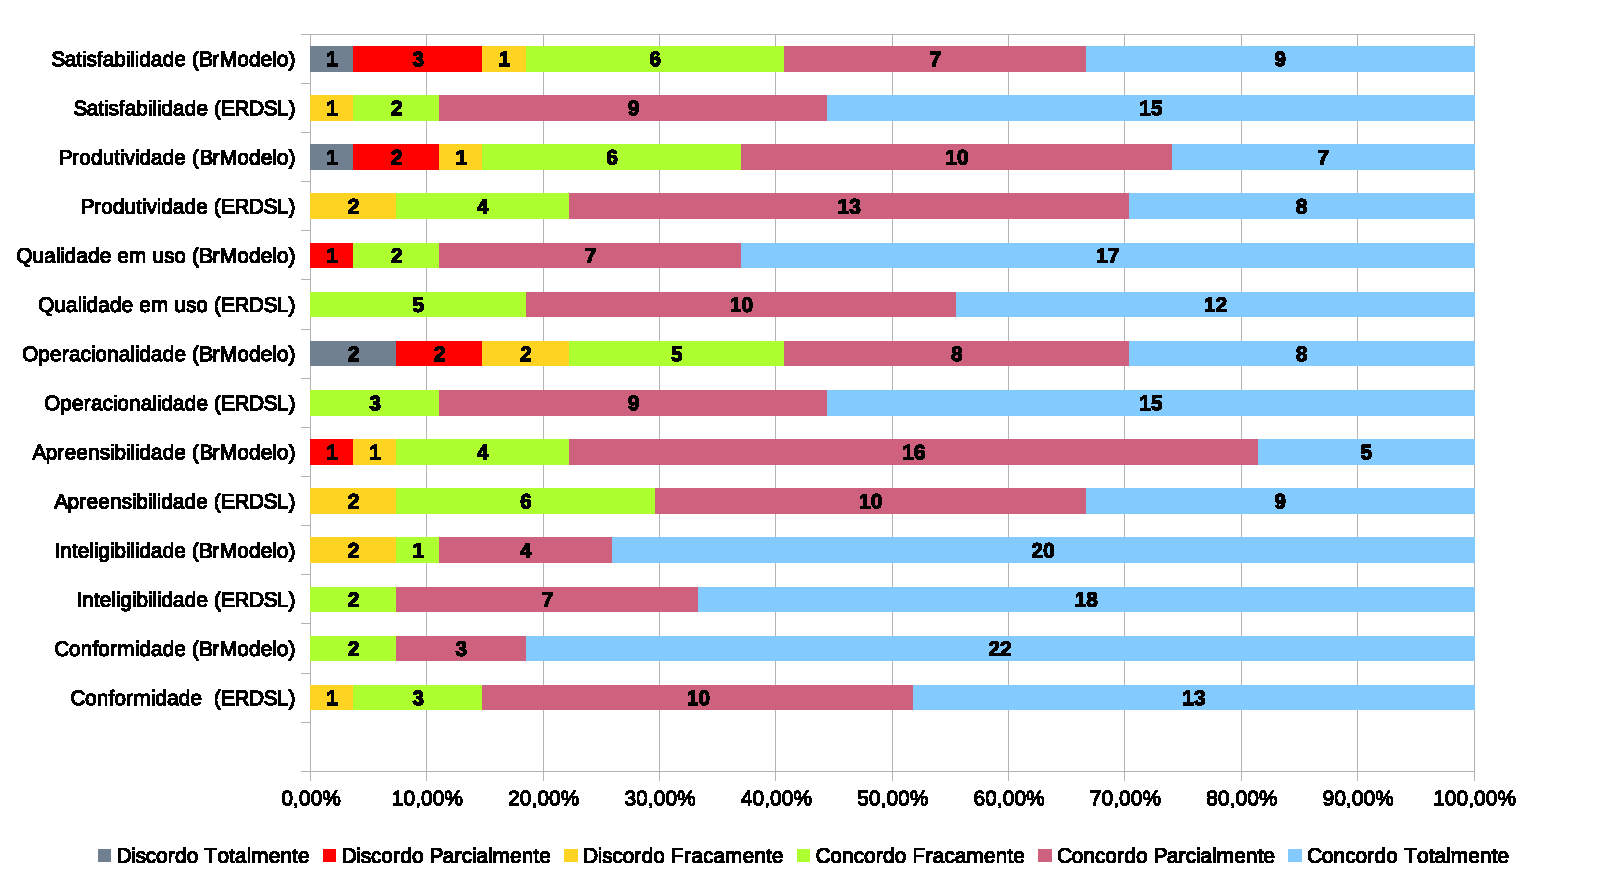
\includegraphics[width=1\textwidth]{img/EPS/Inst3GERAL.eps}
%     \fonte{O autor.}
% \end{figure}

Um ponto que pode ser ressaltado é o conjunto de respostas positivas em relação ao item \textit{Produtividade}, uma vez que no teste de hipótese relativo ao esforço o tratamento utilizando o BrModelo demonstrou uma menor necessidade de tempo para operação.
Na análise dos comentários abertos deste formulário de avaliação, que solicitavam que os participantes indicassem pontos positivos e negativos das ferramentas, foi relatado de forma explícita que a característica de autocomplemento de código proporcionou uma sensação de agilidade no processo de modelagem.

No que diz respeito a \ac{QP}4, sobre a avaliação dos construtores da \ac{DSL}, foram analisados os artefatos do instrumento presente no Apêndice \ref{ap:Inst4Exp}.
Este instrumento listava os oito (8) construtores de modelagem \ac{ER} cobertos pela \ac{DSL}, dispostos com uma escala Likert de um (1) até seis (6).
Novamente, optou-se pele número par na escala para evitar respostas neutras que poderiam levar a uma interpretação mais subjetiva.

Como pode ser observado na \autoref{fig:inst4GERALExp}, que compila todas as respostas recebidas, os construtores relacionados as Entidades e Atributos Descritivos foram os melhores avaliados, com todos os vinte sete (27) concordando com a sua atual representação.

Em contrapartida, todos os outros seis (6) obtiveram ao menos uma avaliação de discordância. 
Nesse sentido, destaca-se os contrutores dos \textit{Relacionamentos Ternários} e das Cardinalidades, com duas (2) e três (3) avaliações discordando das suas atuais representações respectivamente.

\begin{figure}[!htb]
    \centering
    \caption{Avaliação dos construtores da DSL.}
    \label{fig:inst4GERALExp}
    \pgfplotsset{testbar/.style={
            xbar stacked,
            legend cell align=left,
            legend style={
                legend columns=6,
                font=\footnotesize,
                at={(xticklabel cs:1.0)},
                anchor=north east,
                draw=none
                },
            width=10cm,
            axis y line*= none, 
            axis x line*= bottom,
            xmajorgrids = false,
            xmin=0,xmax=27,
            ytick = data,
            yticklabels = {Entidade, Atributo Referencial, Atributo Descritivo, Relação Binária, Relação Ternária, Autorelacionamento, Cardinalidade, Generalização},
            tick align = outside, xtick pos = left,
            bar width=7mm, y=10mm,
            enlarge y limits={abs=0.625},% 0.5 + 0.5*(y - bar width)/y [TeX.sx #47995]
            nodes near coords,
            nodes near coords align=center,%Move values in bar
            every node near coord/.append style={
                black,
                font=\footnotesize,
                text opacity=1,
                fill=white,
                fill opacity=0.5,
                outer sep=\pgflinewidth
            }
        }}
    \begin{tikzpicture}
    \begin{axis}[testbar] 
    \addplot[pattern color=red,pattern=north east lines] coordinates
        {(0,8) (0,7) (0,6) (0,5) (0,4) (0,3) (0,2) (0,1)};
    \addplot[pattern color=teal,pattern=vertical lines] coordinates
        {(0,8) (0,7) (0,6) (0,5) (0,4) (0,3) (0,2) (0,1)};   
    \addplot[pattern color=gray, pattern=grid] coordinates
        {(0,8) (1,7) (0,6) (1,5) (2,4) (1,3) (3,2) (1,1)};   
    \addplot[pattern color=magenta, pattern=north west lines] coordinates
        {(1,8) (2,7) (4,6) (3,5) (9,4) (5,3) (2,2) (2,1)};   
    \addplot[pattern color=blue, pattern=horizontal lines] coordinates
        {(5,8) (6,7) (6,6) (7,5) (7,4) (9,3) (7,2) (7,1)};   
    \addplot[pattern color=green, pattern=crosshatch dots] coordinates
        {(21,8) (18,7) (17,6) (16,5) (9,4) (12,3) (15,2) (17,1)};  
    \legend{1-Discorda, 2, 3, 4, 5, 6-Concorda}
    \end{axis}
    \end{tikzpicture}




% \begin{figure}[!ht]
% \centering
% \caption{Resultados do formulários de avaliação.}
% \begin{tikzpicture}
% \begin{axis}[
%     xbar stacked,
%     legend cell align=center,
%     legend style={
%     legend columns=5,
%         at={(xticklabel cs:1.0)},
%         anchor=north east,
%         draw=none
%     },
%     ytick=data,
%     axis y line*=none,
%     axis x line*=bottom,
%     tick label style={font=\small},
%     legend style={font=\small},
%     label style={font=\small},
%     xtick={0,5,10},
%     xticklabel= {},
%     bar width=7mm,
%     ylabel={Formulário/Grupo},
%     yticklabels={F1-C, F1-E, F2-C, F2-E, F3-C, F3-E},
%     xmin=0,
%     xmax=10,
%     area legend,
%     y=9mm,
%     enlarge y limits={abs=0.825},
%     nodes near coords,
%     nodes near coords align=center,
%     every node near coord/.append style={
%         black,
%         font=\small,
%         text opacity=.65,
%         fill=white,
%         fill opacity=0.6,
%         outer sep=\pgflinewidth
%     }
% ]
% %NOTA 1
% \addplot[pattern color=red,pattern=horizontal lines] coordinates
% {(0,6)(0,5)(0,4)(0,3)(0,2)(0,1)};
% %NOTA 2
% \addplot[pattern color=orange,pattern=grid] coordinates
% {(1,6)(1,5)(1,4)(0,3)(1,2)(0,1)};   
% \addplot[pattern color = green, pattern=crosshatch dots] coordinates
% % NOTA 3
% {(3,6)(3,5)(5,4)(2,3)(5,2)(1,1)};   
% \addplot[pattern color=blue, pattern =vertical lines ] coordinates
% %NOTA 4
% {(2,6)(3,5)(1,4)(4,3)(3,2)(3,1)};   
% \addplot[pattern color=gray, pattern = dots] coordinates
% %NOTA 5
% {(3,6)(3,5)(2,4)(4,3)(0,2)(6,1)};   
% \legend{1-Disagree, 2, 3, 4, 5-Agree}

% \end{axis}
% \end{tikzpicture}
% \footnotesize
% \label{img:respostas1}
% 	\fonte{O autor.}
% \end{figure}
    \fonte{O autor.}
\end{figure}

% \begin{figure}[!htb]
%     \centering
%     \caption{Avaliação dos construtores da \ac{DSL}.}
%     \label{fig:inst4GERALExp}
%     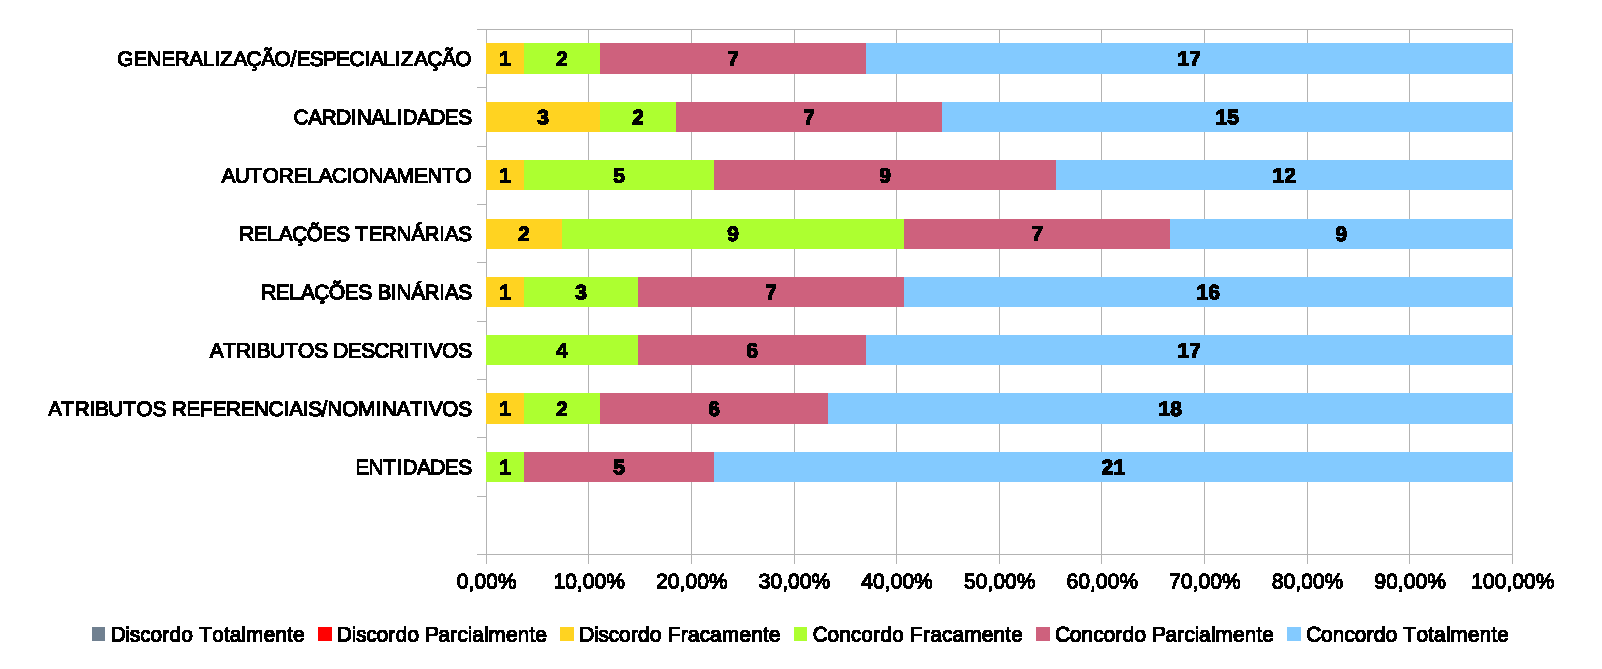
\includegraphics[width=1\textwidth]{img/EPS/Inst4GERAL.eps}
%     \fonte{O autor.}
% \end{figure}

\section{Lições do Capítulo} \label{sec:licoesExp}


Neste capítulo foi apresentado o protocolo e a execução do experimento controlado que foi conduzido para avaliação da proposta deste trabalho.
Para tanto, foram observados fatores como esforço, efetividade, utilidade e facilidade de uso.

Com as respostas obtidas foi possível responder as quatro (4) \acp{QP} do experimento, bem como as duas (2) hipóteses associadas.
A partir da análise feita é possível destacar os seguintes temas:
\begin{itemize}
    \item \textit{Esforço}: a abordagem gráfica para modelagem \ac{ER} mostrou necessitar de menos esforço associado para realizar as tarefas solicitadas, porém considera-se que essa diferença pode ser diminuída com melhorias futuras na ERText;
    \item \textit{Efetividade}: não foi identificado uma diferença média que justifique afirmar que uma abordagem foi melhor do que a outra no que diz respeito a efetividade, entretanto observa-se que existe a necessidade de serem realizados testes que envolvam problemas de complexidades maiores para uma melhor avaliação.
    \item \textit{Comparação qualitativa entre os tratamentos}: foi possível observar que há certo equilíbrio entre os tratamentos, mas destaca-se a avaliação positiva que o atributo \textit{Produtividade} da ERText recebeu dos participantes do experimento. 
    Em razão de ter sido a primeira vez que os sujeitos tiveram contato com a gramática, bem como da ferramenta estar em sua primeira versão, este é um ponto que chama a atenção e merece destaque;
    \item \textit{Avaliação da linguagem proposta}: em decorrência da avaliação dos construtores da \ac{DSL} proposta, existem algumas lacunas quanto ao \textit{design} da linguagem que precisam ser revistos, em especial atenção as cardinalidades e relacionamentos ternários implementados.
    Uma vez que está previsto o prosseguimento do desenvolvimento da linguagem, a execução de uma possível refatoração, e também a implementação de novos construtores, se mostra um passo natural para sua evolução.
\end{itemize}



A partir dos resultados é possível concluir que existe viabilidade para o uso da abordagem textual para modelagem \ac{ER}, uma vez que os resultados não obtiveram diferenças severas no que diz respeito as atividades executadas.
Contudo, com as respostas alcançadas neste experimento verifica-se a necessidade da realização de melhorias, tanto na implementação da ERText quanto no planejamento e execução de um novo experimento controlado.

